% ########################################

\chapter{A Multi-Telescope Observatory}
\label{chap:multiscope}

% ~~~~~~~~~~~~~~~~~~~~

\chaptoc{}

% ########################################

\section{Introduction}
\label{sec:multiscope_intro}

% ~~~~~~~~~~~~~~~~~~~~

\begin{colsection}

In this chapter I describe the potential future expansion of the GOTO project, with additional telescopes at the current site in La Palma and a future second site in Australia.
%
\begin{itemize}
    \item In \nref{sec:multi_tel} I give an outline of the additional work required to create a multi-site scheduling system, and how the existing simulation code can be modified to approximate the required functionality.
    \item In \nref{sec:gw_sims} I describe simulations showing the benefits of additional telescopes observing gravitational-wave alerts in order to locate the counterpart source.
    \item In \nref{sec:survey_sims} I describe further simulations detailing the effects of additional telescopes on the all-sky survey.
\end{itemize}
%
All work described in this chapter is my own unless otherwise indicated, and has not been published elsewhere.

\end{colsection}

% ########################################

\section{Scheduling for multiple telescopes}
\label{sec:multi_tel}

% ~~~~~~~~~~~~~~~~~~~~

\begin{colsection}

As described in \aref{sec:goto_expansion}, the ultimate aim of the GOTO project is to have multiple nodes around the world. Specifically, the plan calls for two full GOTO-8 systems on La Palma and another two at a second site in Australia (either at Siding Spring Observatory in New South Wales or Mt Kent Observatory in Queensland). It is anticipated that the G-TeCS scheduling system described in \aref{sec:observing} will be extended to cover all these telescopes, so that they each query a single observation database and a master scheduler decides what target each telescope should be observing at a given time. This will require a large amount of work to modify both the database structure and the scheduling functions and, as this is not currently implemented into the existing scheduler, several workarounds are needed in order to create realistic multi-telescope simulations.

\end{colsection}

% ~~~~~~~~~~~~~~~~~~~~

\subsection{Multiple observing telescopes}
\label{sec:multi_tel_scheduling}
\begin{colsection}

One of the current restrictions in the scheduling functions (as described in \aref{chap:scheduling}) is that they only ever expect a single pointing in the observation database to be marked as \code{running} at any one time. It is explicitly coded into the scheduler that detecting multiple running pointings should raise a critical error, as certain bugs early in development could lead to this undesired state to occur. Obviously once the system is to be expanded to multiple telescopes this restriction will have to be lifted, but for running simulations a simplification was required to work around it.

It is currently planned that each telescope will have its own pilot and hardware daemons completely independent of each other, with the only point of overlap being the shared scheduler (and, for each site, the conditions daemon). This makes the master scheduler even harder to consider, as each pilot will be querying it completely out-of-sync. If telescope 1 has just finished observing and makes a scheduler check, the scheduler will need to know what telescope 2 is observing, so as not to return the same pointing to telescope 1 (although in some cases having both telescopes observe the same target might be desired, adding yet another level of complexity). But should both telescopes finish observing at the same time then the scheduler will need some way to decide which telescope is assigned which target, perhaps based on the slew time to each target from the telescope's current position.

As none of the above has yet been implemented into the existing code, a simplified system was required in order to simulate multiple telescopes. The existing fake pilot code (described in \aref{sec:goto_sims}) already contains calls to the real scheduling functions, which return the highest priority pointing at given time. The first simplification was to make the function instead return the top $N$ highest pointings, where $N$ is the number of currently observing telescopes. In lieu of any better algorithm to decide which telescope observes which target, the code simply gives the highest priority pointing to telescope 1, the second highest to telescope 2 and so on. Should there only be one valid pointing returned then only telescope 1 will observe, while telescope 2 will remain ``parked'' until it is needed (in practice the second telescope would default to observing the all-sky survey until it also has something to do).

The second simplification was to ensure the telescopes always stay in sync when observing. This was achievable for the simulations described in this chapter because every pointing uses the same exposure set (three \SI{60}{\second} exposures), and therefore they take the same amount of time to observe. However in practice each telescope would take a different amount of time to slew to its target, and so they would quickly get out of sync. Slew time is included in the fake pilot code for each telescope to acquire its new target, and so in order to remain synchronised with multiple telescopes the simulations simply wait the required amount of time for the telescope with the furthest distance to slew. This ensures both telescopes start and finish their observations at the same time, although it does mean a small amount of observing time is ``wasted'' while one telescope is waiting for the other to be in position.

\newpage

\end{colsection}

% ~~~~~~~~~~~~~~~~~~~~
\subsection{Multiple observing sites}
\label{sec:multi_site_scheduling}
\begin{colsection}

The modifications to the scheduler described in the previous section provide a good approximation of the response of an arbitrary number of telescopes observing at one site. However expanding the code further to simulate observations from multiple sites adds further complexity.

The scheduler functions (see \aref{sec:ranking}) need to know which site observations are being made from in order to correctly sort pointings. The visibility constraints (see \aref{sec:constraints}) check if each target is above the local horizon, as well as the local Sun altitude, and the tiebreak parameter (see \aref{sec:breaking_ties}) takes into account the airmass of each target. These are simple parameters to calculate if you have only one site observing at once, but once there are telescopes at multiple sites querying the scheduler at the same time then the responses will need to take the position of each into account.

This could lead to problems when returning the highest priority pointings. For example, with two telescopes observing from different sites the scheduler could return the highest priority pointing visible from each. If they are different then each telescope can then observe the best target for its site; however if both telescopes were observing at the same time, and the visible portions of the sky from both sites overlapped, then it is very possible that the same pointing would be the highest priority from both sites. Assuming they should not both observe the same target at the same time, the scheduler would need to chose which telescope to assign that pointing to and then recalculate a different target for the other telescope. What would be better is to use the same method described in \aref{sec:multi_tel_scheduling}, and have the scheduler always return the top $X$ pointings, where $X = N_\text{site1} + N_\text{site2} + \cdots$ is the total number of telescopes across the globe. In reality targets would need to be assigned to telescopes based on their airmass at each site, or the slew time from the current target, but as in \aref{sec:multi_tel_scheduling} for the simulations they can just be assigned to each telescope in order.

\newpage

\begin{figure}[t]
    \begin{center}
        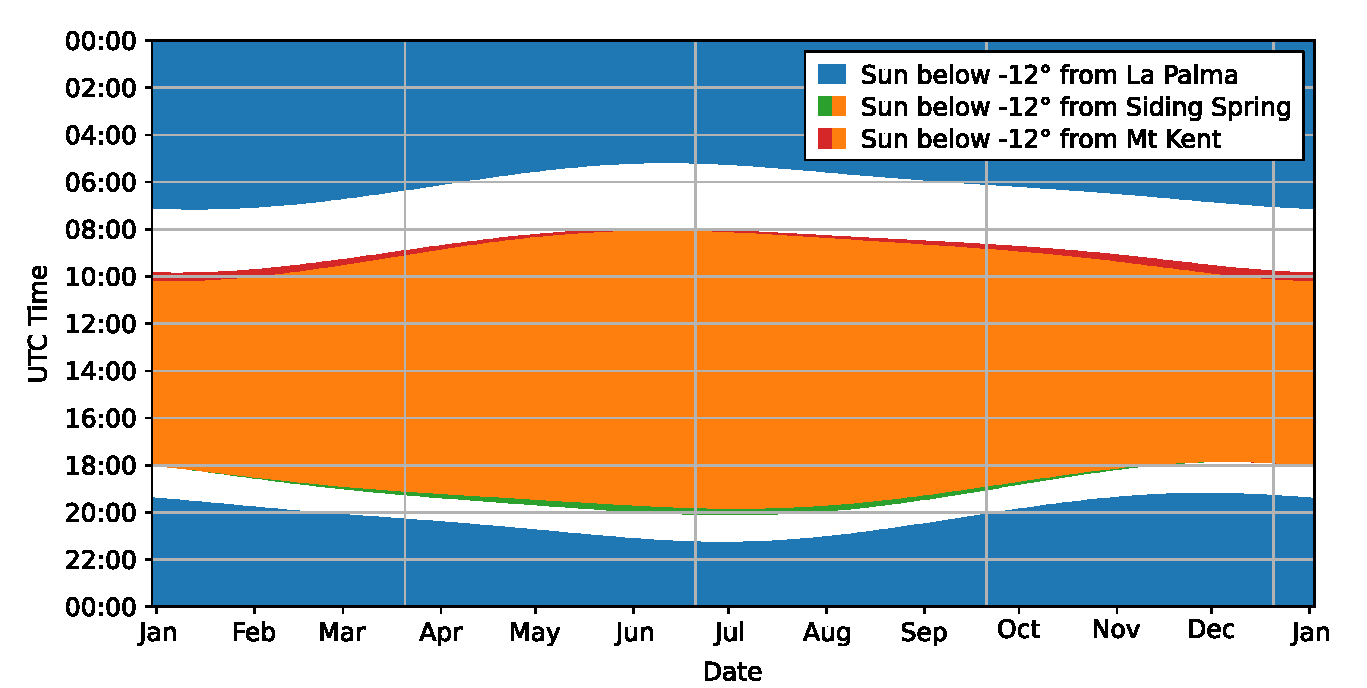
\includegraphics[width=\linewidth]{images/nights.pdf}
    \end{center}
    \caption[Night times throughout the year for GOTO sites]{
        Night times throughout the year for GOTO sites. Night here is defined as when the Sun is \SI{12}{\degree} below the local horizon.
    }\label{fig:nights}
\end{figure}

However, saying that the scheduler needs to find the top $X$ pointings, where $X$ is the total number of telescopes at all sites, is not strictly true --- it actually only needs to return enough pointings to satisfy the telescopes at the sites that are currently observing. In other words, if there are two sites but one is shut down, due to weather or because it is daytime there, the scheduler only needs to consider the single site. Conveniently for simulating the proposed GOTO network this is always true, by defining night as when the Sun is below \SI{-12}{\degree} the periods of darkness between La Palma and either of the two proposed Australian sites never overlap. This is shown in \aref{fig:nights}, where there is a constant ``buffer zone'' between night ending at one site and beginning at the other. This case only applies for a very limited number of combinations of sites. As shown in \aref{fig:site_nights} there is a tear-drop-shaped area on the Earth's surface which contain the locations where the local night will never overlap with night on La Palma, comprising only of eastern Australia, New Zealand and Melanesia. For a Sun altitude limit of \SI{-12}{\degree} below the horizon this area contains just $6.6 \%$ of the Earth's surface.

\begin{figure}[p]
    \begin{center}
        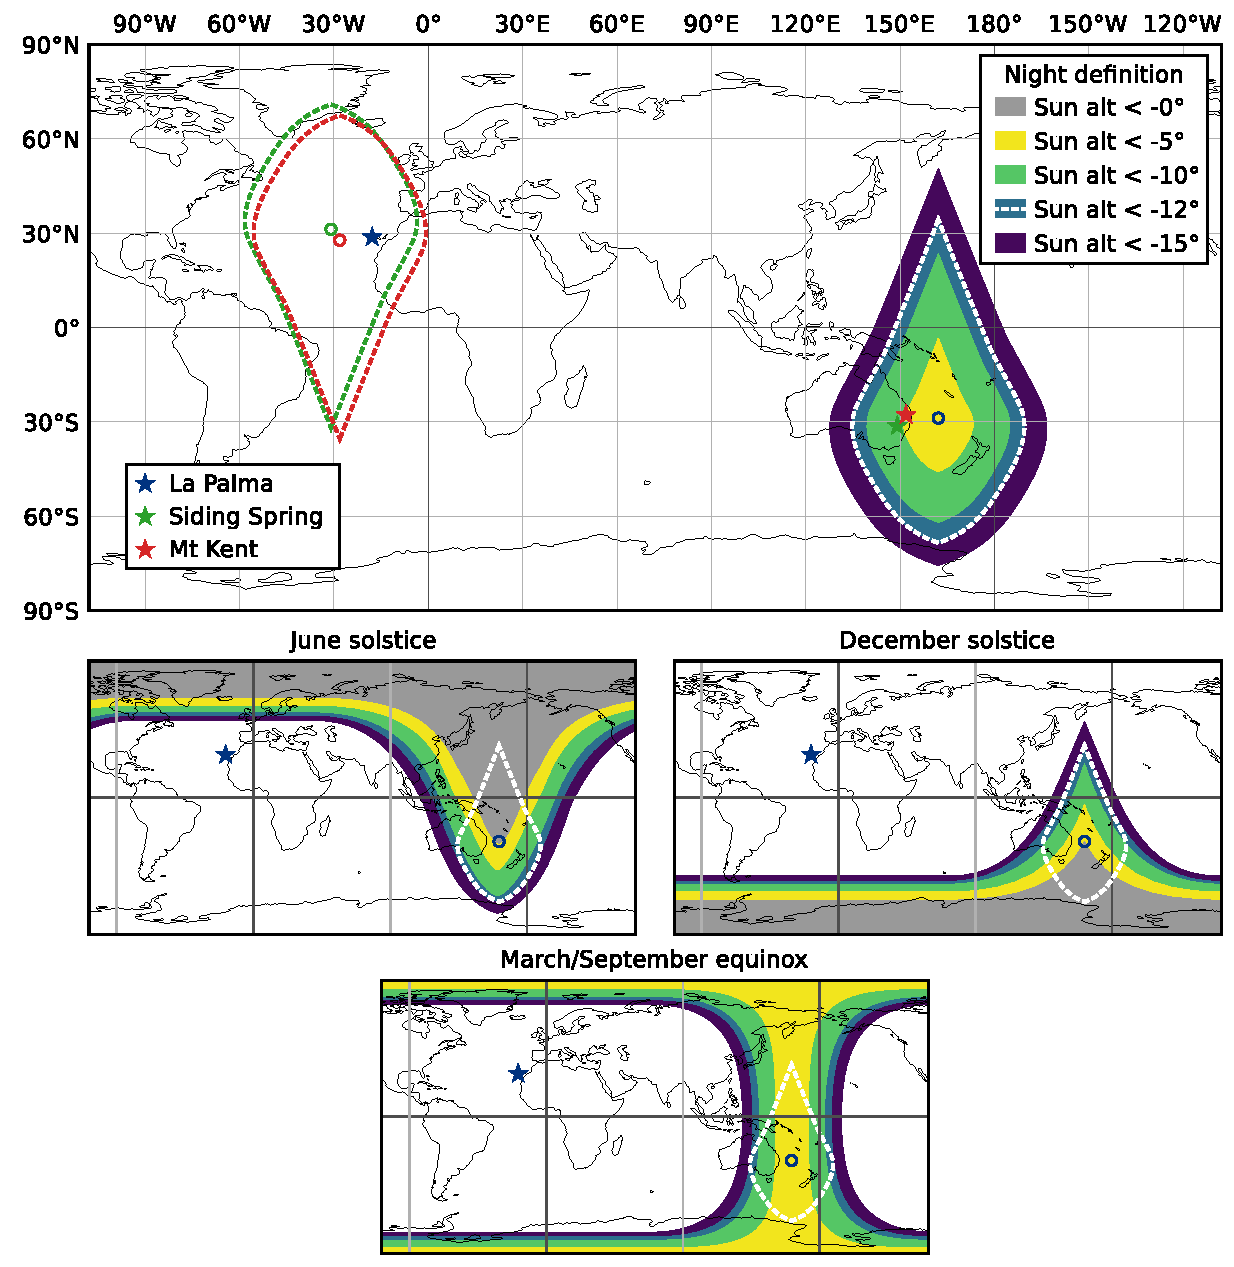
\includegraphics[width=\linewidth]{images/sites.pdf}
    \end{center}
    \caption[Locations on the Earth with non-overlapping night times]{
        Finding locations on the Earth with non-overlapping night times. In the upper plot the filled areas show the locations on the Earth where local night never overlaps with night on La Palma, at any time of the year. The different colours denote different night time definitions, with the \SI{-12}{\degree} definition also being surrounded by a white dashed line. The location of the GOTO sites considered (\textcolor{NavyBlue}{La Palma}, \textcolor{Green}{Siding Spring} and \textcolor{Red}{Mt Kent}) are marked with stars and their antipodes are marked with hollow circles. The equivalent areas for Siding Spring and Mt Kent are also shown by the coloured dashed lines surrounding their antipodes, for the \SI{-12}{\degree} night definition only. The lower plots show how the region varies over the course of a year, from the solstices via the equinox (the plot is identical for the two equinoxes and therefore is only shown once).
    }\label{fig:site_nights}
\end{figure}

The fortuitous location of the proposed Australian sites means implementing telescopes at multiple sites into the simulation code was fairly simple. Each simulation would consider either only La Palma or La Palma and one of the Australian sites, as these are the only anticipated scenarios for GOTO.\@ In the two-site cases only the telescopes at one of the sites would ever be observing at any one time, and so the simulation only requires the multi-telescope implementation as described in \aref{sec:multi_tel_scheduling}.

Should simulations be desired for other sites on the Earth that are not within the small area with non-overlapping nights shown in \aref{fig:site_nights}, for example other potential GOTO-South sites in South Africa or Chile, then the simulation code would need to be modified to take this into account. This has not yet been done as it was not required for the scenarios described here. In principle the fact the sites overlap could be ignored, and the simulations can be run for each site as a stand-alone observatory and then combined afterwards with the results from other, stand-alone simulations. This however removes the benefit of the sites acting together and using a common observation database, and would lead to multiple observations of the same targets from each site.

\end{colsection}

% ~~~~~~~~~~~~~~~~~~~~

\subsection{Simulating different survey grids}
\label{sec:multi_grid_scheduling}
\begin{colsection}

One fundamental feature of the existing G-TeCS code is that observations are carried out on a fixed all-sky grid, as defined in \aref{chap:tiling}. When considering multiple telescopes this is both useful in some ways and limiting in others. Having a fixed grid that is common to all telescopes is vital for the GOTO image subtraction pipeline GOTOphoto, as it requires observations of the same part of the sky to create reference frames for difference imaging (see \aref{sec:gotophoto}). This is why a common grid is anticipated to form the base of the global system. By sharing the same tiles each telescope can contribute to the same all-sky survey grid, as well as efficiently coordinate mapping out a gravitational-wave skymap.

\newpage

However, sharing the grid requires all of the telescopes to have essentially the same field of view. There is some leeway in the exact field of view of each telescope array; the grid tiles are defined to leave a slight overlap around the edge (see \aref{fig:4ut_footprint}). But if the field of view of the telescope array is much larger than the tile size then the pointings will be too close together and therefore inefficient. Even worse, if the field of view of the telescope array is much smaller than the defined tile size it would lead to gaps in the sky coverage.

For the proposed GOTO system with near-identical GOTO-8 units around the world this is not an issue, but it should be recognised as a limitation of not just the simulations but the whole G-TeCS control system. One potential case where this may be an issue is when commissioning GOTO-South. If it spends time as a GOTO-4 system similar to La Palma before getting the second set of unit telescopes to bring it up to a full set of eight, then it will be observing concurrently with one or two GOTO-8 systems on La Palma. This is a likely enough situation that it was considered in the gravitational-wave simulations as described in \aref{sec:gw_sims}, using the work around of two independent simulations mentioned previously. How this scenario would be dealt with within a real implementation of G-TeCS is a problem that needs development in the future, should it prove to be necessary.

\end{colsection}

% ########################################

\section{Gravitational-wave follow-up simulations}
\label{sec:gw_sims}

% ~~~~~~~~~~~~~~~~~~~~

\begin{colsection}

As the primary mission of the GOTO project is to follow up gravitational-wave detections, it is important to consider what benefit additional telescopes will bring to the project. In order to do this, simulations were run on the LIGO First Two Years mock skymaps \citep{First2Years}, a small selection of which were previously used for the scheduler simulations described in \aref{sec:scheduler_sims}. The full sample contained 1105 events, each based on simulating a binary neutron star coalescence at a particular sky position and distance. Each event had two skymaps generated: the first using the rapid BAYESTAR pipeline \citep{BAYESTAR}, which is typically available minutes after the event, and the second using the LALInference code \citep{LALInference} which can take hours or days to complete. For these simulations, therefore, only the BAYESTAR skymaps were considered in order to focus on GOTO's initial follow-up, although an extension to the simulations could include the effects of the second updated skymap being processed and added to the database some hours after the event.

\end{colsection}

% ~~~~~~~~~~~~~~~~~~~~

\subsection{Event visibility}
\label{sec:gw_visability}
\begin{colsection}

The simulations were designed to begin at the time the event was detected, and then simulate the next 24 hours of observations. This guaranteed one night's worth of observing at each site, although split into two halves if the event occurred during the night. The time each event occurred was taken from the simulated skymaps, and does not account for the delay between the event being detected and the alert being issued and processed by the G-TeCS sentinel. Events were uniformly distributed in time of occurrence during the day, and they all occurred over a two month period spanning either side of the 2010 September equinox as shown in \aref{fig:f2y_times}. It is not clear why this range of dates was selected, although surrounding one of the equinoxes might have been an attempt to reduce bias towards observers from either hemisphere. Detailed analysis shows the events are not entirely equally distributed either side of the equinox (03:09 on 2010--09--23), with the first event occurring 33 days before the equinox and the last 27 days after. Overall 64\% of events occurred before the September equinox and 36\% after, which leads to a slight bias in visibility towards southern telescopes as they experience longer nights before the equinox (in the southern winter).

\begin{figure}[t]
    \begin{center}
        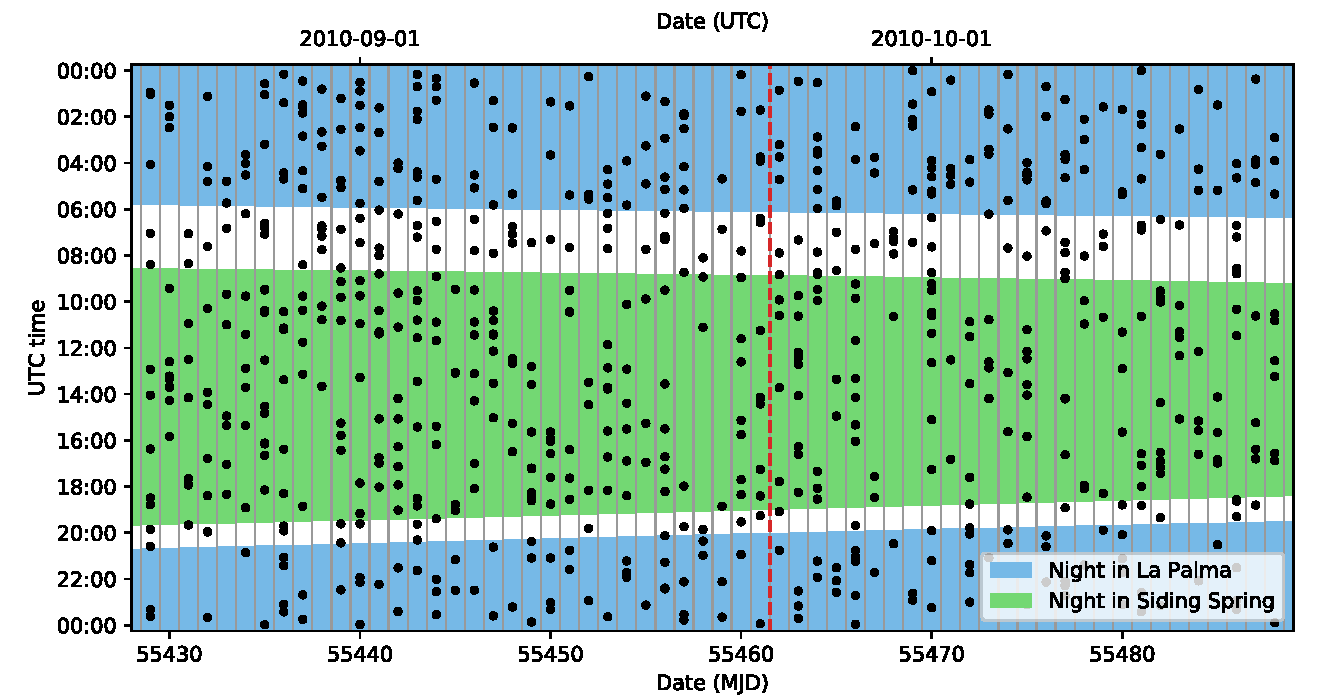
\includegraphics[width=\linewidth]{images/f2y_times.pdf}
    \end{center}
    \caption[Date and time distribution of events in the First Two Years sample]{
        Date and time distribution of the ``First Two Years'' events. The night periods are shown in \textcolorbf{NavyBlue}{blue} for La Palma and \textcolorbf{Green}{green} for Siding Spring, and the date of the equinox is marked by the \textcolorbf{Red}{red} dashed line.
    }\label{fig:f2y_times}
\end{figure}

Events were uniformly distributed across the sky, and are uniform in distance cubed \citep{First2Years}. Although each source included distance information this was not taken into account in the simulations aside from determining the event strategy to use (all were well within the \SI{400}{\mega\parsec} definition for close neutron star events defined for GOTO-alert in \aref{sec:event_strategy}). Future simulations could use the distance to the event to estimate a light curve based on the observed kilonova for GW170817 \citep{GW170817_followup} and use it to predict how long each event would be visible for GOTO for (the GW170817 transient AT 2017gfo faded below GOTO's 20 mag limit after 2.5 days).

\newpage

The first stage of simulating observations of each event was to determine if the source location was visible from the chosen site(s) in the 24 hours after the event occurred. In the cases where this was not true there was no point running the full simulation, as it the source would never be observed. Each event was classified into one of four categories: % chktex 36

\begin{itemize}
    \item \textbf{Not visible --- too close to the Sun}. These events had sources that were too close to the Sun to observe within the 24 hour period after the event, regardless of the site considered. This was defined as the source location being within \SI{42}{\degree} of the Sun (\SI{-12}{\degree} from the definition of night time plus \SI{30}{\degree} from the altitude limit). It is a fixed fraction of the sky: 5280 sq deg or 13\% of the celestial sphere\footnote{The area of a circle with radius $r$ on the surface of a sphere with radius $R$ is $2\pi R^2(1-\cos(r))$. The radius of the celestial sphere $R=\SI{360}{\degree}/2\pi \approx \SI{57.3}{\degree}$.}.

    \item \textbf{Not visible --- below declination limit}. The sources for these events fell within the region of the sky that is never visible due to the limited declination range visible from a given site. For example, using the GOTO \SI{30}{\degree} altitude limit a telescope on La Palma (latitude \SI{28}{\degree} N) can see a band of sky between \SI{+88}{\degree} and \SI{-32}{\degree} declination. Sources outside of this region (that are not already excluded due to being too close to the Sun) would therefore never be observable from the site, but could be observed from other locations. At the equator this band covers 87\% of the sky over the course of a year, at latitudes of $\pm \SI{30}{\degree}$ 75\% of the sky is visible, falling to just 25\% at the poles\footnote{The area of a segment on a sphere between angles $\theta$ and $\phi$ is $2 \pi R^2 (\cos(\theta)-\cos(\phi))$}.

    \item \textbf{Not visible --- daytime}. These event sources are sufficiently far enough from the Sun and are within the visible declination range, but are still not observable from a given site during the 24 hour period after the event. This includes the region of the sky that is technically visible from the site, only while the Sun is still above the \SI{-12}{\degree} horizon. Unlike the fraction of the sky within \SI{42}{\degree} of the Sun these positions could still be observable from other sites at different latitudes.

    \item \textbf{Visible}. The source for this event falls outside of either of the above three areas, and therefore is nominally above the \SI{30}{\degree} altitude limit at some point during night time within 24 hours after the event. The portion of the sky that is visible in one night from a given site depends on the latitude of the site and the time of year.
\end{itemize}

\begin{table}[t]
    \begin{center}
        \begin{tabular}{c|ccc} % chktex 44
            \multirow{3}{*}{Night} & \multicolumn{3}{c}{Site} \\
                      & La Palma             & Siding Spring  & Mt Kent \\
                      & (\SI{28}{\degree} N) &  (\SI{31}{\degree} S) &  (\SI{27}{\degree} S) \\
                      \midrule
                      \\
            March     & \textcolorbf{Green}{57.1\% visible}
                      & \textcolorbf{Green}{56.3\% visible}
                      & \textcolorbf{Green}{59.6\% visible}
                      \\
            equinox   & {\scriptsize(\textcolorbf{Orange}{12.9\%} $\cdot$
                                     \textcolorbf{NavyBlue}{23.4\%} $\cdot$
                                     \textcolorbf{Blue}{6.7\%})}
                      & {\scriptsize(\textcolorbf{Orange}{12.9\%} $\cdot$
                                     \textcolorbf{NavyBlue}{24.6\%} $\cdot$
                                     \textcolorbf{Blue}{6.2\%})}
                      & {\scriptsize(\textcolorbf{Orange}{12.9\%} $\cdot$
                                     \textcolorbf{NavyBlue}{22.5\%} $\cdot$
                                     \textcolorbf{Blue}{5.0\%})}
                      \\[0.5cm]
            June      & \textcolorbf{Green}{50.4\% visible}
                      & \textcolorbf{Green}{61.9\% visible}
                      & \textcolorbf{Green}{62.7\% visible}
                      \\
            solstice  & {\scriptsize(\textcolorbf{Orange}{12.9\%} $\cdot$
                                     \textcolorbf{NavyBlue}{24.2\%} $\cdot$
                                     \textcolorbf{Blue}{12.4\%})}
                      & {\scriptsize(\textcolorbf{Orange}{12.9\%} $\cdot$
                                     \textcolorbf{NavyBlue}{20.9\%} $\cdot$
                                     \textcolorbf{Blue}{4.3\%})}
                      & {\scriptsize(\textcolorbf{Orange}{12.9\%} $\cdot$
                                     \textcolorbf{NavyBlue}{19.0\%} $\cdot$
                                     \textcolorbf{Blue}{5.4\%})}
                      \\[0.5cm]
            September & \textcolorbf{Green}{57.0\% visible}
                      & \textcolorbf{Green}{56.4\% visible}
                      & \textcolorbf{Green}{57.7\% visible}
                      \\
            equinox   & {\scriptsize(\textcolorbf{Orange}{12.9\%} $\cdot$
                                     \textcolorbf{NavyBlue}{23.4\%} $\cdot$
                                     \textcolorbf{Blue}{6.7\%})}
                      & {\scriptsize(\textcolorbf{Orange}{12.9\%} $\cdot$
                                     \textcolorbf{NavyBlue}{24.5\%} $\cdot$
                                     \textcolorbf{Blue}{6.2\%})}
                      & {\scriptsize(\textcolorbf{Orange}{12.9\%} $\cdot$
                                     \textcolorbf{NavyBlue}{22.4\%} $\cdot$
                                     \textcolorbf{Blue}{7.0\%})}
                      \\[0.5cm]
            December  & \textcolorbf{Green}{62.5\% visible}
                      & \textcolorbf{Green}{48.9\% visible}
                      & \textcolorbf{Green}{51.0\% visible}
                      \\
            solstice  & {\scriptsize(\textcolorbf{Orange}{12.9\%} $\cdot$
                                     \textcolorbf{NavyBlue}{19.7\%} $\cdot$
                                     \textcolorbf{Blue}{4.8\%})}
                      & {\scriptsize(\textcolorbf{Orange}{12.9\%} $\cdot$
                                     \textcolorbf{NavyBlue}{25.8\%} $\cdot$
                                     \textcolorbf{Blue}{12.4\%})}
                      & {\scriptsize(\textcolorbf{Orange}{12.9\%} $\cdot$
                                     \textcolorbf{NavyBlue}{23.2\%} $\cdot$
                                     \textcolorbf{Blue}{12.9\%})}
                      \\
        \end{tabular}
    \end{center}
    \caption[Sky visibility over a year]{
        Sky visibility over a year from the three different GOTO sites. The upper value in \textcolorbf{Green}{green} shows the fraction of the sky that is visible during the night. The lower values break down the remaining fraction of the sky into the three non-visible categories: too close to the Sun in \textcolorbf{Orange}{orange}, below the declination limit in \textcolorbf{NavyBlue}{light blue} and only visible during the day in \textcolorbf{Blue}{dark blue}.
    }\label{tab:visibility}
\end{table}

The region of the sky visible during the night for a given site change over the course of the year. \aref{tab:visibility} shows the fractions of the sky in each of the four categories above at the solstices and equinoxes. \aref{fig:visibility} plots the regions on the celestial sphere, in order to better visualise how they change depending on observing site and time of year.

\begin{figure}[p]
    \begin{center}
        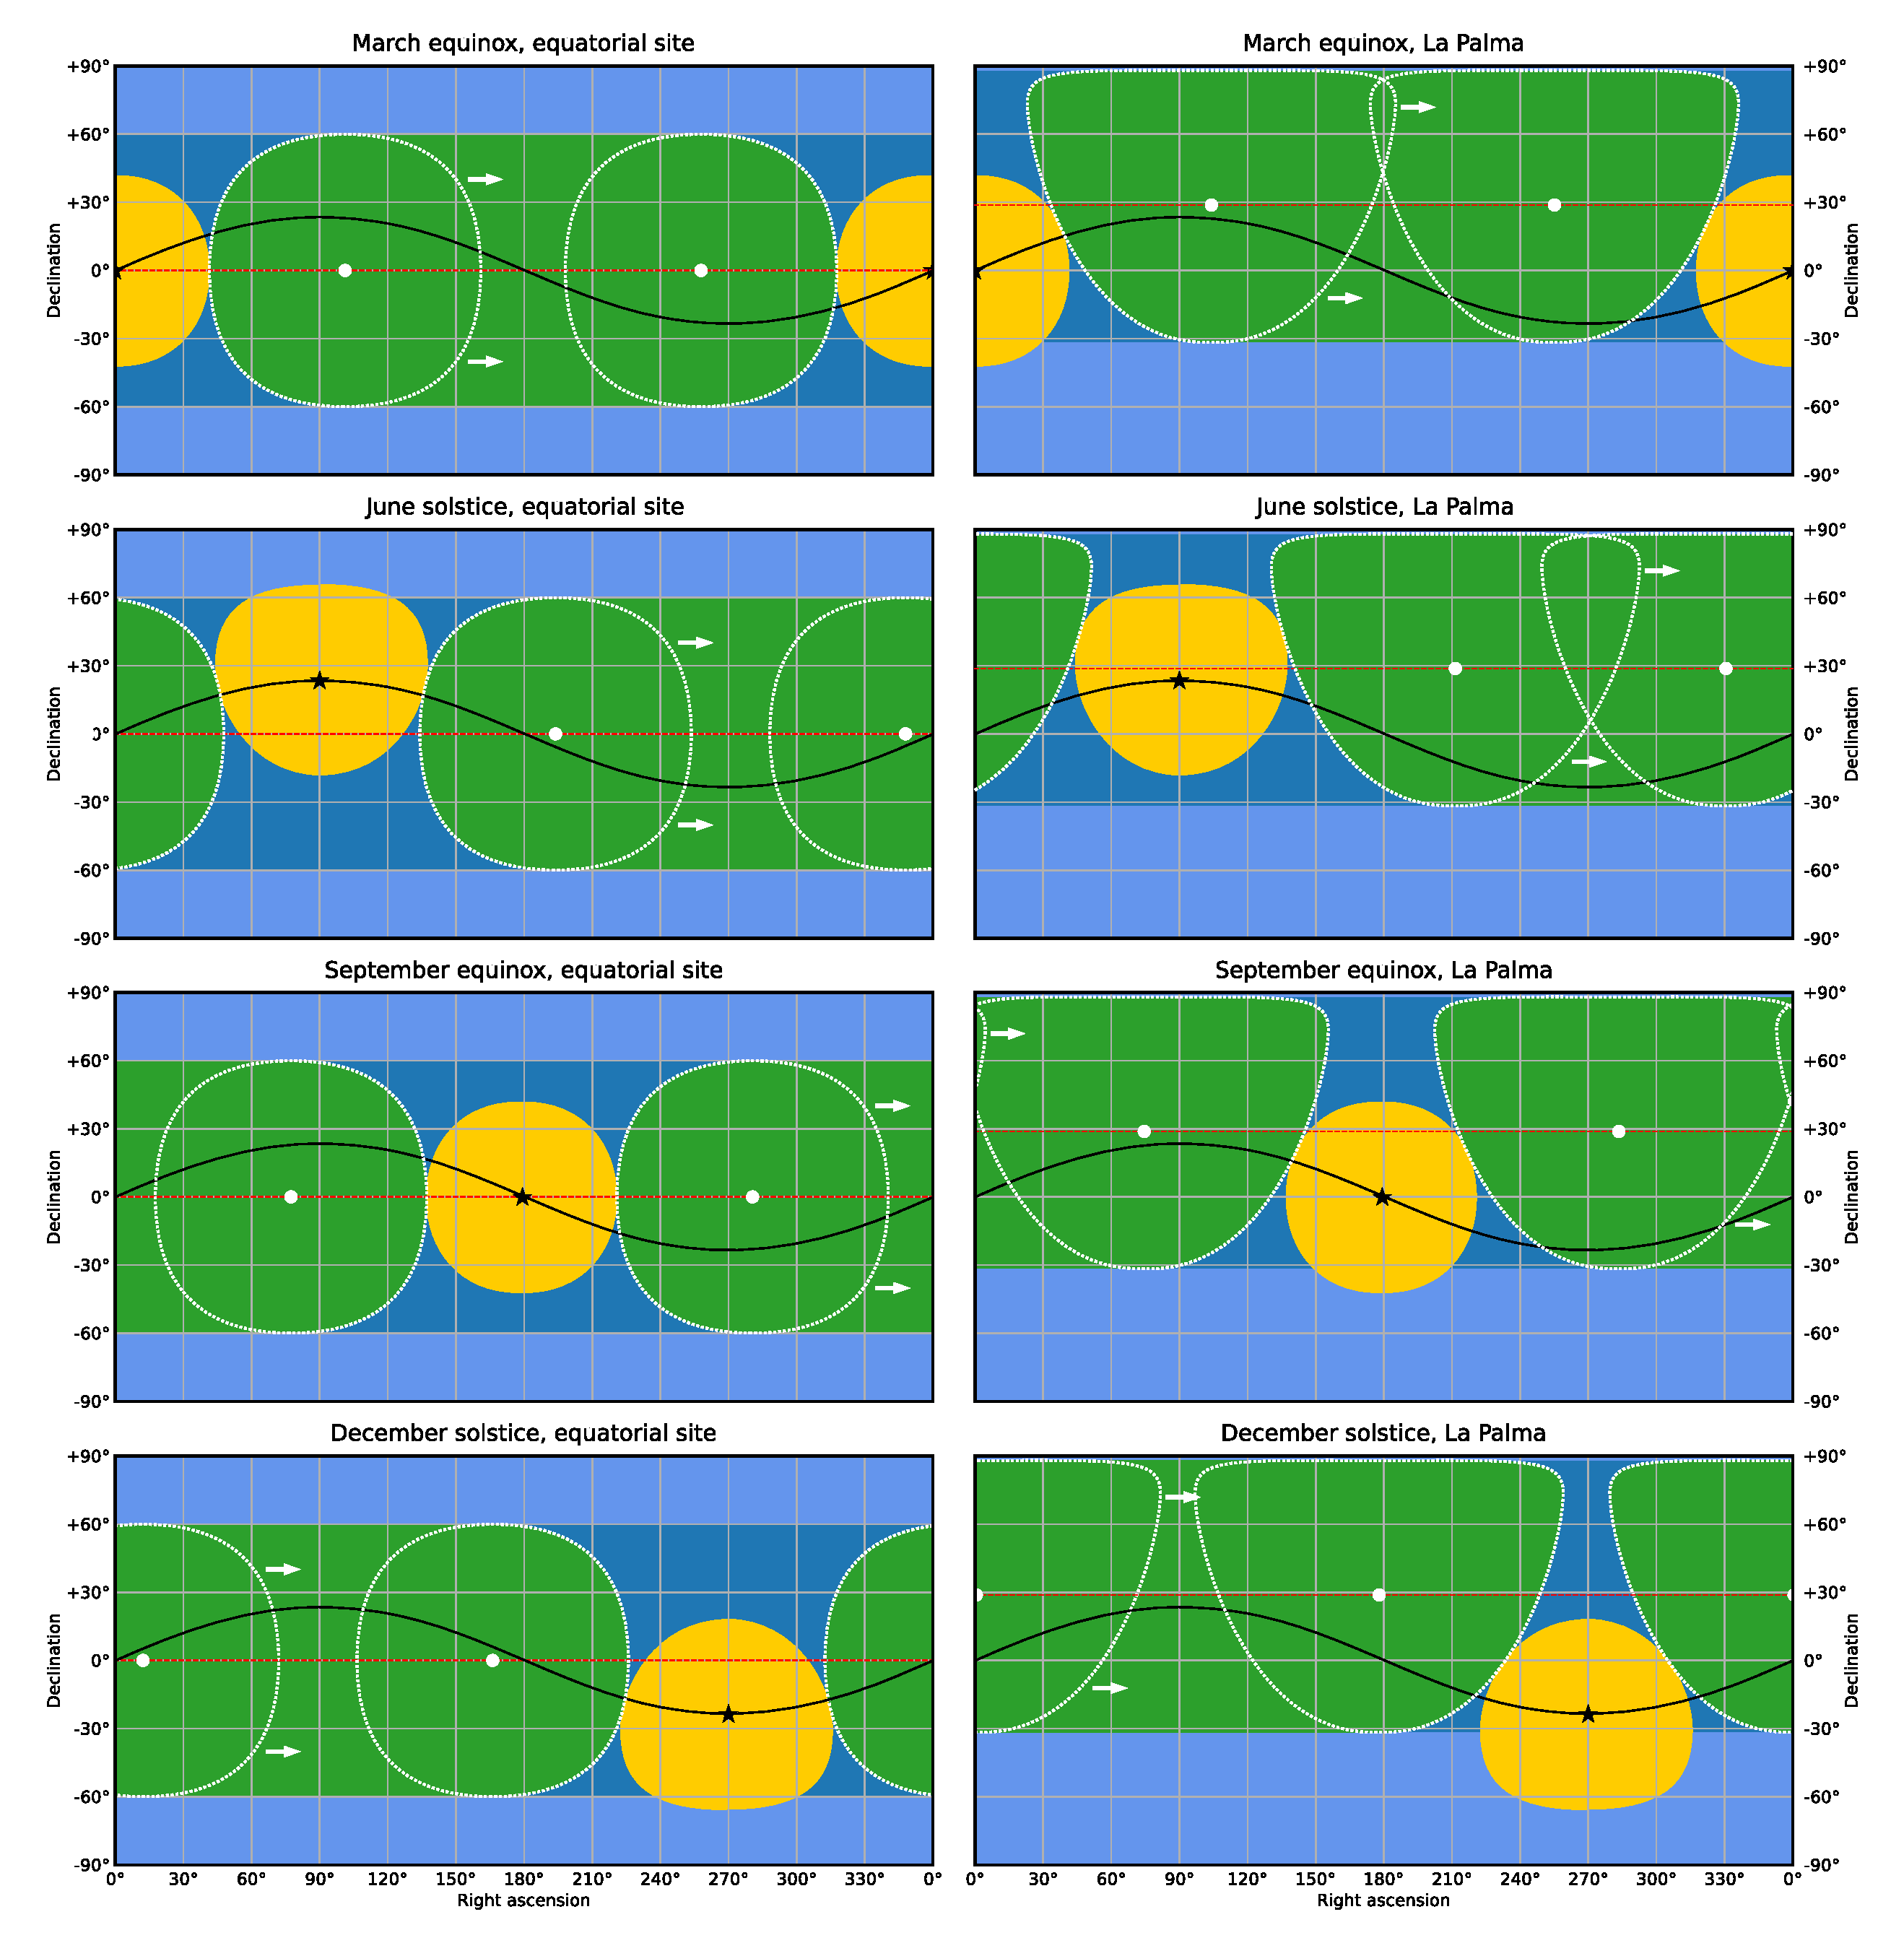
\includegraphics[width=\linewidth]{images/visibility.pdf}
    \end{center}
    \caption[Plotting sky visibility regions over a year]{
        Changing sky visibility regions over a year, plotted on the celestial sphere.
        Visibility is shown at the equinoxes and the solstices for two different sites: the left column shows visibility for an observer located on the Earth's equator, the right column shows visibility from La Palma. The \textcolorbf{Green}{green} regions are visible during the night. The area above the \SI{30}{\degree} altitude limit at sunset is shown by a white dashed line, with the local zenith marked with a white point, and the arrows show how the visible region moves in RA during the night until sunrise. The position of the Sun on the ecliptic is shown by the black star, the \textcolorbf{Orange}{orange} region is within \SI{42}{\degree} of the Sun and is therefore not visible from anywhere on Earth. The \textcolorbf{NavyBlue}{light blue} regions are permanently out of the visible declination range of the site, and the regions in \textcolorbf{Blue}{dark blue} would only be visible during the day.
    }\label{fig:visibility}
\end{figure}

\clearpage

\end{colsection}

% ~~~~~~~~~~~~~~~~~~~~

\subsection{Selecting event tiles}
\label{sec:gw_selecting}
\begin{colsection}

Even if the source of a gravitational-wave event is visible within 24 hours from a given site (or combination of sites) there is one further criterion that would prevent observations of the source --- whether or not the source is located within any of the tile pointings added to the database. The issue of determining which tiles to add to the database is detailed in \aref{sec:event_insert}, but is ultimately a matter of probability: if a telescope covers the 90\% confidence region for every gravitational-wave event then it would be expected to observe 90\% of the sources.

GOTO-alert uses the mean contour level method to select tiles, as described in \aref{sec:event_insert}. For simulations described in this chapter a mean contour selection value of $0.9$ was used for the GOTO-4 grid and $0.95$ for the GOTO-8 grid. Using these values 92\% of GW events had sources within at least one of the selected tiles for the GOTO-4 grid, and 95\% for the GOTO-8 grid. Two events where the source location was outside of the selected tiles are shown in \aref{fig:poor_selection}. In the following simulation results the tile selection was only considered after the visibility restrictions in the previous section had been applied, as the visibility would be true for any telescopes at the relevant sites while the tiles are specific to GOTO.\@ In other words, if the source location was visible but was not within the tiles selected by GOTO that is only GOTO's problem, and other telescopes might still have observed it.

In order to find the optimal selection levels, further simulations could be run using the same sample of skymaps but altering the selection level. As discussed in \aref{sec:event_insert} there is a trade-off between adding too few tiles and missing the source, and adding too many and increasing the time to cover them all. Additional telescopes in the GOTO network would lead to the skymap being covered faster, which could make adding less probable tiles worthwhile.

\begin{figure}[p]
    \begin{center}
        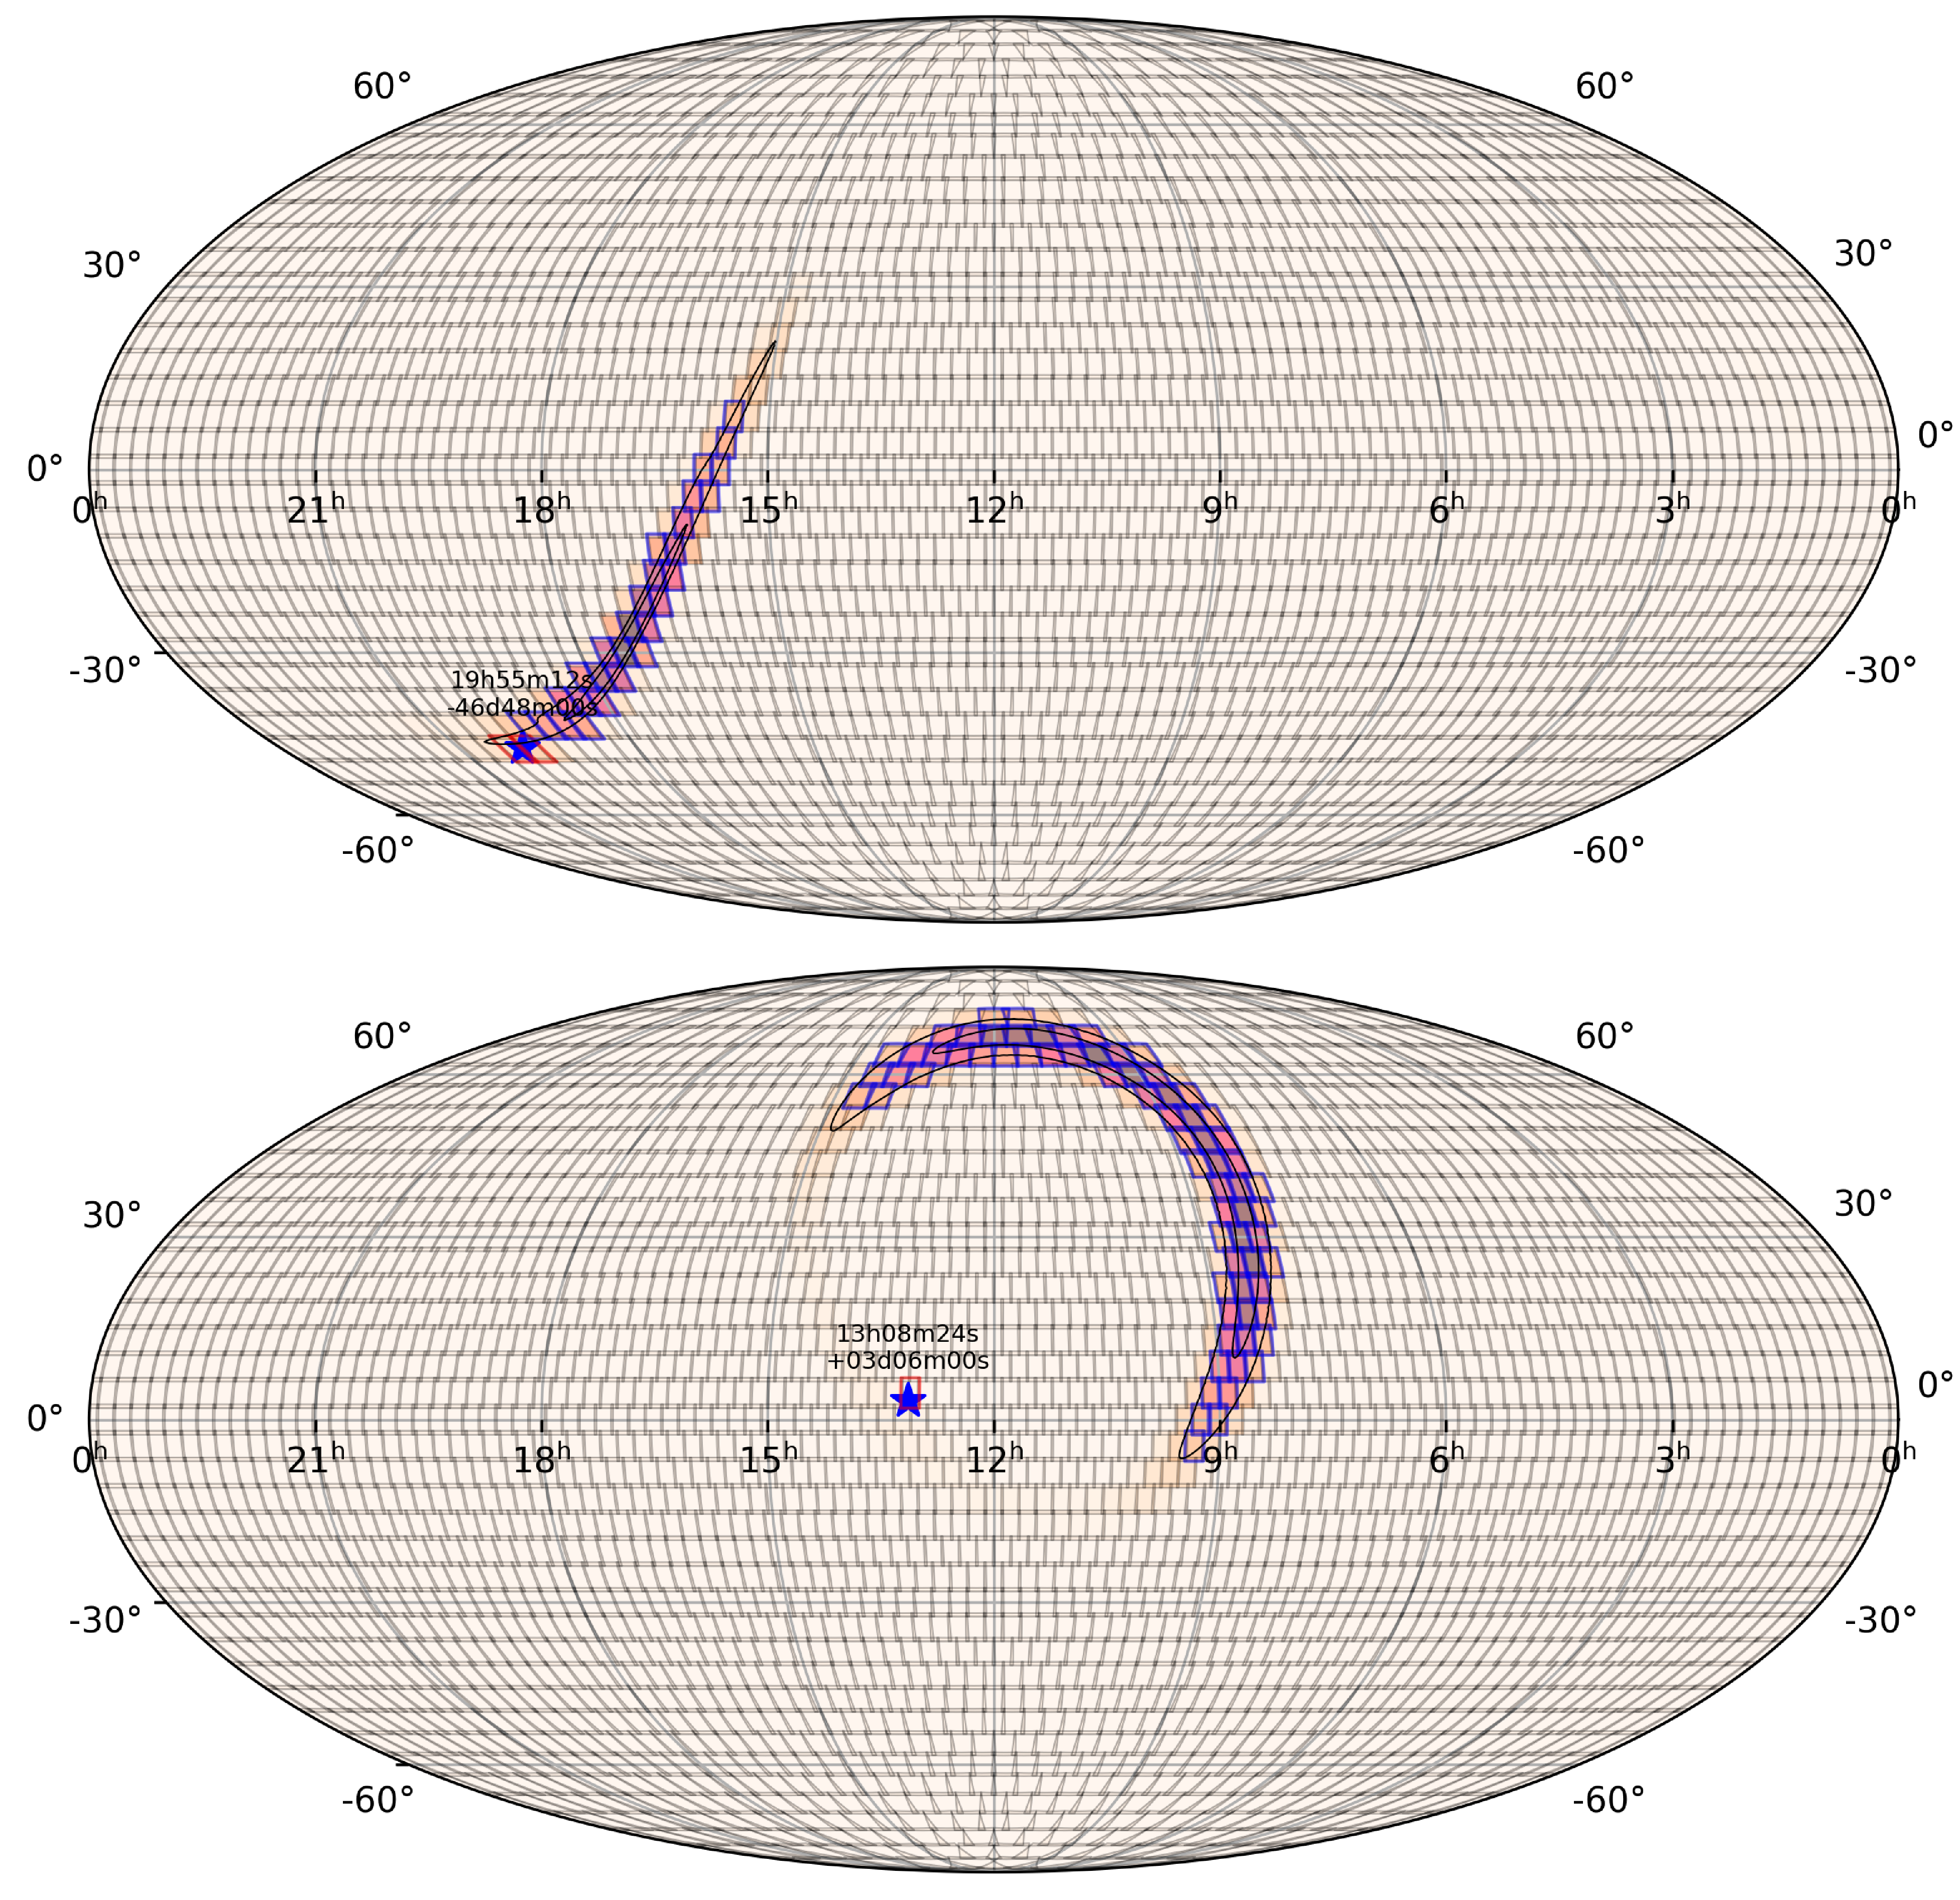
\includegraphics[width=\linewidth]{images/non_selected.pdf}
    \end{center}
    \caption[Examples of mock GW event sources falling outside of the selected tiles]{
        Two examples of mock GW event sources (marked by the \textcolorbf{Red}{red} star) falling outside the selected tiles (the tiles highlighted in \textcolorbf{NavyBlue}{blue}). In the upper case (trigger ID 13630) the source fell just outside of the selected tiles, while in the lower case (trigger ID 930001) the source was on completely the other side of the sky.
    }\label{fig:poor_selection}
\end{figure}

\clearpage

\end{colsection}

% ~~~~~~~~~~~~~~~~~~~~

\subsection{Multi-telescope simulation results}
\label{sec:gw_sim_results}
\begin{colsection}

In order to simulate the response of different GOTO systems, each of the 1105 First Two Years skymaps \citep{First2Years} were simulated using a script \code{sim\_skymaps.py}. The object of the simulations was to find how quickly the event source would be observed. For events that fell into one of the exceptions described above, either the source was not visible within 24 hours or the source tile was not selected to be added to the database, the simulation was aborted early and the result recorded. The remaining events were classified as ``observable'', and for these the full fake pilot simulation was run for up to 24 hours after the time the event occurred. The fake pilot knew which tiles the event source fell within, and once any of those tiles were recorded as being observed the simulation ended. The time of the observation, as well as the position and time the tile was observed was recorded. Any events which were simulated for the full 24 hours without the source being observed were counted as failures and were classed as ``not observed''.

Simulations were carried out for a variety of possible GOTO systems. Each simulation was assigned a code based on how many telescopes of each type were located at each site. Two possible GOTO ``models'' were considered: the GOTO-4 prototype with four unit telescopes and the intended GOTO-8 design with eight (see \aref{sec:goto_design}). In the following section the code \textbf{1N4} refers to one GOTO-4 mount in La Palma (the current system at the time of writing), \textbf{2N8+1S4} is two GOTO-8 telescopes on La Palma and one GOTO-4 in Siding Spring, \textbf{2N8+1K4} would be the same but the southern telescope is at Mt Kent.

The results of the simulations for six key scenarios are given in the following plots: \aref{fig:gw_sim_1n4}, \aref{fig:gw_sim_1n8} and \aref{fig:gw_sim_2n8} show results for the evolving site on La Palma, while \aref{fig:gw_sim_2n8+1s4}, \aref{fig:gw_sim_2n8+2s8} and \aref{fig:gw_sim_2n8+2k8} shows the effect of adding three different southern facilities. A summary of the key results from all of the simulations that have been carried out is given in \aref{tab:gw_sim_results}.

\newpage

\begin{figure}[p]
    \begin{center}
        \begin{minipage}[t]{0.15\linewidth}\vspace{0.6cm}
            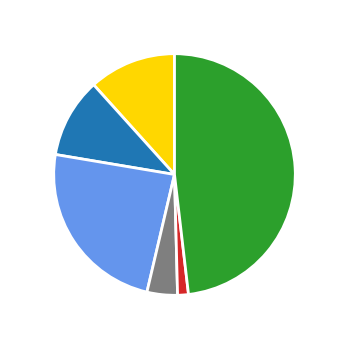
\includegraphics[trim={.5cm 0 .5cm 0},clip,width=\linewidth]{images/gw_sims/1n4_pie.png}
        \end{minipage}
        \begin{minipage}[t]{0.45\linewidth}\vspace{0pt}
            \begin{tabular}{lrr}
                \multicolumn{3}{c}{\textbf{Simulation results}} \\
                \midrule
                %% PASTE BELOW \/\/
                \textcolor{Green}{Observed} & 532 & 48.1\% \\
                \textcolor{Red}{Not observed} & 16 & 1.4\% \\
                \textcolor{darkgray}{Not selected} & 45 & 4.1\% \\
                \textcolor{NavyBlue}{Never above dec limit} & 265 & 24.0\% \\
                \textcolor{Blue}{Not visible at night} & 118 & 10.7\% \\
                \textcolor{Orange}{Too close to Sun} & 129 & 11.7\% \\
                \midrule
                Visible events & 593 &  53.7\% \\
                %% PASTE ABOVE /\/\
            \end{tabular}
        \end{minipage}
        \begin{minipage}[t]{0.37\linewidth}\vspace{0pt}
            \begin{tabular}{lr}
                \multicolumn{2}{c}{\textbf{System: 1N4}} \\
                \midrule
                %% PASTE BELOW \/\/
                Observing efficiency & 89.7\% \\
                \midrule
                Mean delay after     & \multirow{2}{*}{9.96 h} \\
                event time           & \\
                Mean delay after     & \multirow{2}{*}{1.58 h} \\
                becoming visible     & \\
                \midrule
                Mean airmass         & 1.64 \\
                %% PASTE ABOVE /\/\
            \end{tabular}
        \end{minipage}
    \end{center}
    \caption[GW simulation results: 1N4 system]{
        Simulation results for a 1N4 system. The pie chart and the table on the left shows which category each of the 1105 events fell into. ``Visible events'' includes only the top three categories, and the ``observing efficiency'' is the fraction of these events which were subsequently observed. The table on the right gives the mean delay and airmass of the source observation, for events where the source was observed.
    }\label{fig:gw_sim_1n4}
\end{figure}

\begin{figure}[p]
    \begin{center}
        \begin{minipage}[t]{0.15\linewidth}\vspace{0.6cm}
            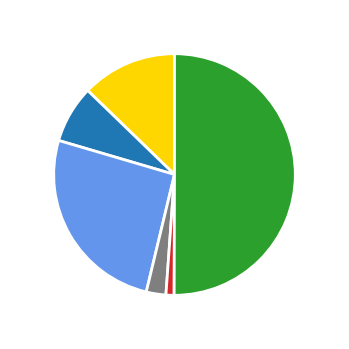
\includegraphics[trim={.5cm 0 .5cm 0},clip,width=\linewidth]{images/gw_sims/1n8_pie.png}
        \end{minipage}
        \begin{minipage}[t]{0.45\linewidth}\vspace{0pt}
            \begin{tabular}{lrr}
                \multicolumn{3}{c}{\textbf{Simulation results}} \\
                \midrule
                %% PASTE BELOW \/\/
                \textcolor{Green}{Observed} & 553 & 50.0\% \\
                \textcolor{Red}{Not observed} & 12 & 1.1\% \\
                \textcolor{darkgray}{Not selected} & 29 & 2.6\% \\
                \textcolor{NavyBlue}{Never above dec limit} & 285 & 25.8\% \\
                \textcolor{Blue}{Not visible at night} & 85 & 7.7\% \\
                \textcolor{Orange}{Too close to Sun} & 141 & 12.8\% \\
                \midrule
                Visible events & 594 &  53.8\% \\
                %% PASTE ABOVE /\/\
            \end{tabular}
        \end{minipage}
        \begin{minipage}[t]{0.37\linewidth}\vspace{0pt}
            \begin{tabular}{lr}
                \multicolumn{2}{c}{\textbf{System: 1N8}} \\
                \midrule
                %% PASTE BELOW \/\/
                Observing efficiency & 93.1\% \\
                \midrule
                Mean delay after     & \multirow{2}{*}{10.06 h} \\
                event time           & \\
                Mean delay after     & \multirow{2}{*}{1.60 h} \\
                becoming visible     & \\
                \midrule
                Mean airmass         & 1.66 \\
                %% PASTE ABOVE /\/\
                & \\
            \end{tabular}
        \end{minipage}
    \end{center}
    \caption[GW simulation results: 1N8 system]{
        Simulation results for a 1N8 system. Note the distribution of events changes due to the different grid used, and the biggest gain in events observed is from the decreased number with sources not included in the selected tiles.
    }\label{fig:gw_sim_1n8}
\end{figure}

\begin{figure}[p]
    \begin{center}
        \begin{minipage}[t]{0.15\linewidth}\vspace{0.6cm}
            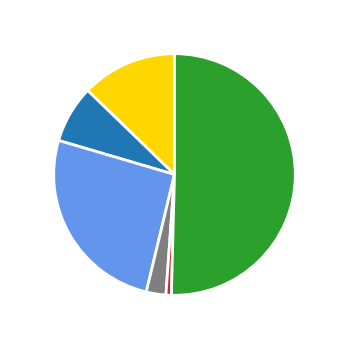
\includegraphics[trim={.5cm 0 .5cm 0},clip,width=\linewidth]{images/gw_sims/2n8_pie.png}
        \end{minipage}
        \begin{minipage}[t]{0.45\linewidth}\vspace{0pt}
            \begin{tabular}{lrr}
                \multicolumn{3}{c}{\textbf{Simulation results}} \\
                \midrule
                %% PASTE BELOW \/\/
                \textcolor{Green}{Observed} & 557 & 50.4\% \\
                \textcolor{Red}{Not observed} & 8 & 0.7\% \\
                \textcolor{darkgray}{Not selected} & 29 & 2.6\% \\
                \textcolor{NavyBlue}{Never above dec limit} & 285 & 25.8\% \\
                \textcolor{Blue}{Not visible at night} & 85 & 7.7\% \\
                \textcolor{Orange}{Too close to Sun} & 141 & 12.8\% \\
                \midrule
                Visible events & 594 &  53.8\% \\
                %% PASTE ABOVE /\/\
            \end{tabular}
        \end{minipage}
        \begin{minipage}[t]{0.37\linewidth}\vspace{0pt}
            \begin{tabular}{lr}
                \multicolumn{2}{c}{\textbf{System: 2N8}} \\
                \midrule
                %% PASTE BELOW \/\/
                Observing efficiency & 93.8\% \\
                \midrule
                Mean delay after     & \multirow{2}{*}{9.89 h} \\
                event time           & \\
                Mean delay after     & \multirow{2}{*}{1.53 h} \\
                becoming visible     & \\
                \midrule
                Mean airmass         & 1.67 \\
                %% PASTE ABOVE /\/\
                & \\
            \end{tabular}
        \end{minipage}
    \end{center}
    \caption[GW simulation results: 2N8 system]{
        Simulation results for a 2N8 system. The improvements over the 1N8 system are a small gain in observing efficiency and a decrease in the mean delay time.
    }\label{fig:gw_sim_2n8}
\end{figure}

\newpage

\begin{figure}[p]
    \begin{center}
        \begin{minipage}[t]{0.15\linewidth}\vspace{0.6cm}
            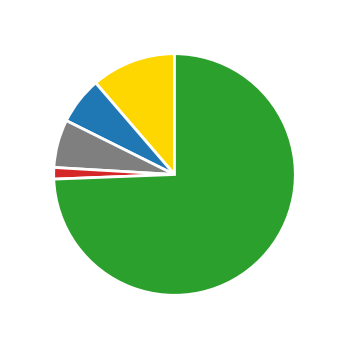
\includegraphics[trim={.5cm 0 .5cm 0},clip,width=\linewidth]{images/gw_sims/2n8&1s4_pie.png}
        \end{minipage}
        \begin{minipage}[t]{0.45\linewidth}\vspace{0pt}
            \begin{tabular}{lrr}
                \multicolumn{3}{c}{\textbf{Simulation results}} \\
                \midrule
                %% PASTE BELOW \/\/
                \textcolor{Green}{Observed} & 822 & 74.4\% \\
                \textcolor{Red}{Not observed} & 17 & 1.5\% \\
                \textcolor{darkgray}{Not selected} & 71 & 6.4\% \\
                \textcolor{NavyBlue}{Never above dec limit} & 0 & 0.0\% \\
                \textcolor{Blue}{Not visible at night} & 70 & 6.3\% \\
                \textcolor{Orange}{Too close to Sun} & 125 & 11.3\% \\
                \midrule
                Visible events & 910 &  82.4\% \\
                %% PASTE ABOVE /\/\
            \end{tabular}
        \end{minipage}
        \begin{minipage}[t]{0.37\linewidth}\vspace{0pt}
            \begin{tabular}{lr}
                \multicolumn{2}{c}{\textbf{System: 2N8+1S4}} \\
                \midrule
                %% PASTE BELOW \/\/
                Observing efficiency & 90.3\% \\
                \midrule
                Mean delay after     & \multirow{2}{*}{8.16 h} \\
                event time           & \\
                Mean delay after     & \multirow{2}{*}{1.66 h} \\
                becoming visible     & \\
                \midrule
                Mean airmass         & 1.63 \\
                %% PASTE ABOVE /\/\
                & \\
            \end{tabular}
        \end{minipage}
    \end{center}
    \caption[GW simulation results: 2N8+1S4 system]{
        Simulation results for a 2N8+1S4 system. As these sites use different grids they were simulated independently and the results combined.
    }\label{fig:gw_sim_2n8+1s4}
\end{figure}

\begin{figure}[p]
    \begin{center}
        \begin{minipage}[t]{0.15\linewidth}\vspace{0.6cm}
            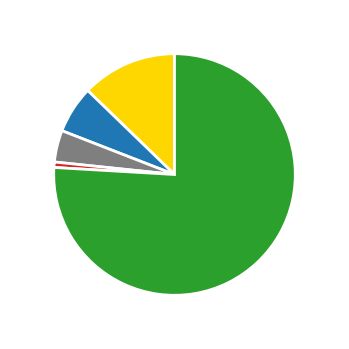
\includegraphics[trim={.5cm 0 .5cm 0},clip,width=\linewidth]{images/gw_sims/2n8+2s8_pie.png}
        \end{minipage}
        \begin{minipage}[t]{0.45\linewidth}\vspace{0pt}
            \begin{tabular}{lrr}
                \multicolumn{3}{c}{\textbf{Simulation results}} \\
                \midrule
                %% PASTE BELOW \/\/
                \textcolor{Green}{Observed} & 839 & 75.9\% \\
                \textcolor{Red}{Not observed} & 8 & 0.7\% \\
                \textcolor{darkgray}{Not selected} & 47 & 4.3\% \\
                \textcolor{NavyBlue}{Never above dec limit} & 0 & 0.0\% \\
                \textcolor{Blue}{Not visible at night} & 70 & 6.3\% \\
                \textcolor{Orange}{Too close to Sun} & 141 & 12.8\% \\
                \midrule
                Visible events & 894 &  80.9\% \\
                %% PASTE ABOVE /\/\
            \end{tabular}
        \end{minipage}
        \begin{minipage}[t]{0.37\linewidth}\vspace{0pt}
            \begin{tabular}{lr}
                \multicolumn{2}{c}{\textbf{System: 2N8+2S8}} \\
                \midrule
                %% PASTE BELOW \/\/
                Observing efficiency & 93.8\% \\
                \midrule
                Mean delay after     & \multirow{2}{*}{7.69 h} \\
                event time           & \\
                Mean delay after     & \multirow{2}{*}{1.57 h} \\
                becoming visible     & \\
                \midrule
                Mean airmass         & 1.64 \\
                %% PASTE ABOVE /\/\
                & \\
            \end{tabular}
        \end{minipage}
    \end{center}
    \caption[GW simulation results: 2N8+2S8 system]{
        Simulation results for a 2N8+2S8 system. The obvious improvement over the northern hemisphere-only 2N8 system (\aref{fig:gw_sim_2n8}) is the removal of the declination-limited events, meaning more event sources are visible. The observing efficiency remains the same, but there is a notable improvement in the post-event delay times.
    }\label{fig:gw_sim_2n8+2s8}
\end{figure}

\begin{figure}[p]
    \begin{center}
        \begin{minipage}[t]{0.15\linewidth}\vspace{0.6cm}
            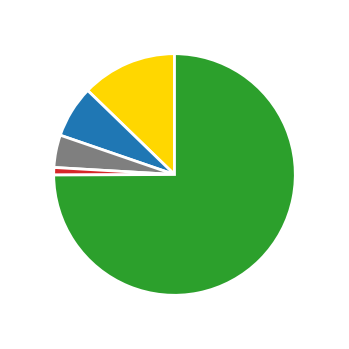
\includegraphics[trim={.5cm 0 .5cm 0},clip,width=\linewidth]{images/gw_sims/2n8+2k8_pie.png}
        \end{minipage}
        \begin{minipage}[t]{0.45\linewidth}\vspace{0pt}
            \begin{tabular}{lrr}
                \multicolumn{3}{c}{\textbf{Simulation results}} \\
                \midrule
                %% PASTE BELOW \/\/
                \textcolor{Green}{Observed} & 828 & 74.9\% \\
                \textcolor{Red}{Not observed} & 11 & 1.0\% \\
                \textcolor{darkgray}{Not selected} & 48 & 4.3\% \\
                \textcolor{NavyBlue}{Never above dec limit} & 0 & 0.0\% \\
                \textcolor{Blue}{Not visible at night} & 77 & 7.0\% \\
                \textcolor{Orange}{Too close to Sun} & 141 & 12.8\% \\
                \midrule
                Visible events & 887 &  80.3\% \\
                %% PASTE ABOVE /\/\
            \end{tabular}
        \end{minipage}
        \begin{minipage}[t]{0.37\linewidth}\vspace{0pt}
            \begin{tabular}{lr}
                \multicolumn{2}{c}{\textbf{System: 2N8+2K8}} \\
                \midrule
                %% PASTE BELOW \/\/
                Observing efficiency & 93.3\% \\
                \midrule
                Mean delay after     & \multirow{2}{*}{7.69 h} \\
                event time           & \\
                Mean delay after     & \multirow{2}{*}{1.55 h} \\
                becoming visible     & \\
                \midrule
                Mean airmass         & 1.64 \\
                %% PASTE ABOVE /\/\
                & \\
            \end{tabular}
        \end{minipage}
    \end{center}
    \caption[GW simulation results: 2N8+2K8 system]{
        Simulation results for a 2N8+2K8 system. Comparing to \aref{fig:gw_sim_2n8+2s8} it makes very little difference to the results if the southern site is at Siding Spring or Mt Kent, when compared to the huge gain from having either available instead of just La Palma (\aref{fig:gw_sim_2n8}).
    }\label{fig:gw_sim_2n8+2k8}
\end{figure}

\begin{table}[p]
    \begin{center}
        \begin{tabular}{c|cccc|c|cc} % chktex 44
            \multirow{2}{*}{System} &
            \multicolumn{4}{c|}{Source observed within \ldots} &
            {\small Observing} &
            \multicolumn{2}{c}{Mean delay after \ldots} \\
                & 1h & 6h & 12h & 24h & efficiency & {\small the event} & {\small becoming visible} \\
            \midrule
                 1N4 &  5.9\% & 16.5\% & 26.2\% & 48.1\% & 89.7\% &  9.96 h & 1.58 h \\
                 1N8 &  6.8\% & 16.9\% & 27.1\% & 50.0\% & 93.1\% & 10.06 h & 1.60 h \\
                 2N8 &  7.2\% & 17.3\% & 27.9\% & 50.4\% & 93.8\% &  9.89 h & 1.53 h \\
            &&&&&&&\\
                 1S4 &  8.8\% & 18.8\% & 27.9\% & 47.1\% & 87.7\% &  9.39 h & 1.64 h \\
                 1S8 & 10.3\% & 20.6\% & 31.1\% & 49.2\% & 91.0\% &  8.81 h & 1.52 h \\
                 2S8 & 11.1\% & 21.2\% & 31.8\% & 49.9\% & 92.1\% &  8.67 h & 1.47 h \\
            &&&&&&&\\
                 2K8 & 10.8\% & 20.9\% & 31.3\% & 50.9\% & 92.3\% &  9.02 h & 1.46 h \\
            &&&&&&&\\
             1N8+1S8 & 17.1\% & 36.8\% & 52.5\% & 74.8\% & 92.5\% &  7.82 h & 1.63 h \\
             2N8+1S8 & 17.6\% & 37.2\% & 52.9\% & 75.2\% & 93.0\% &  7.75 h & 1.59 h \\
             2N8+2S8 & 18.4\% & 37.7\% & 53.8\% & 75.9\% & 93.8\% &  7.69 h & 1.57 h \\
            &&&&&&&\\
            2N8+2K8  & 18.2\% & 38.0\% & 52.8\% & 74.9\% & 93.3\% &  7.69 h & 1.55 h \\
            &&&&&&&\\
            2N8+1S4* & 16.0\% & 35.7\% & 50.3\% & 74.4\% & 90.3\% &  8.16 h & 1.66 h \\
            2N8+1S8* & 17.6\% & 37.2\% & 53.0\% & 75.2\% & 93.0\% &  7.76 h & 1.60 h \\
            2N8+2S8* & 18.4\% & 37.7\% & 53.7\% & 75.9\% & 93.8\% &  7.70 h & 1.58 h \\
        \end{tabular}
    \end{center}
    \caption[GW simulation results summary table]{
        Summary of simulation results. The fraction of events where the source was observed is given for different time delays after the event, along with the overall observing efficiency after 24 hours. The mean delay between the event and the source being observed is given, along with the mean time it took to observe the source tile after it became visible. Systems marked with an asterisk (*) were not simulated together, but were instead combined from the individual simulations for each site.
    }\label{tab:gw_sim_results}
\end{table}

\clearpage

\end{colsection}

% ~~~~~~~~~~~~~~~~~~~~

\subsection{Analysis of simulation results}
\label{sec:gw_sim_analysis}
\begin{colsection}

The results of the gravitational-wave follow-up simulations support two conclusions: the addition of the southern site provides a huge benefit to the number of sources that can be observed, while adding further telescopes at a single site provides a much more modest benefit. \aref{fig:gw_sim_results} summarises the simulated post-event delay times for the different possible stages of GOTO deployment.

\begin{figure}[t]
    \begin{center}
        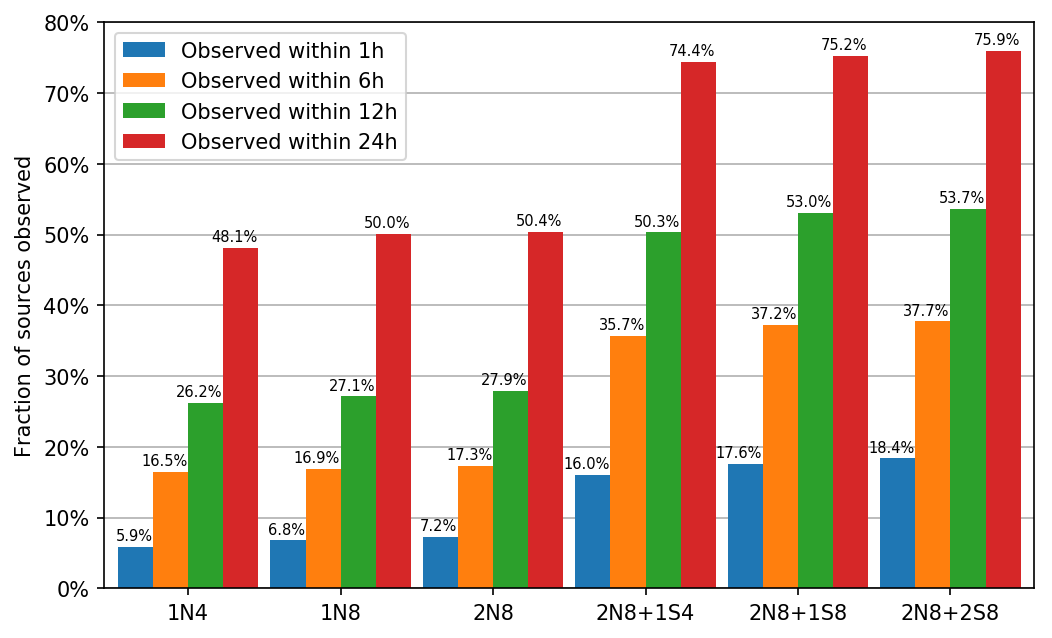
\includegraphics[width=\linewidth]{images/gw_sims/results.png}
    \end{center}
    \caption[Simulation delay time for different GOTO systems]{
        Post-event delay in observing gravitational-wave event sources for six possible deployment stages of the GOTO system.
    }\label{fig:gw_sim_results}
\end{figure}

The reason for the first conclusion is obvious: adding a site in the southern hemisphere opens up a large number of sources that are physically incapable of being observed from La Palma. The second comes about essentially because the efficiency of a single GOTO system is already very high. \aref{fig:gw_sim_1n8} shows that the 1N8 system already observes 93.1\% of all sources visible from La Palma, and the majority of those not observed were outside of the selected tiles (29 events) compared to just not being observed (12 events). The addition of the second GOTO-8 system as shown in \aref{fig:gw_sim_2n8} moves just 4 events from ``not observed'' to ``observed'', the addition of a second telescope can not make any changes to any of the other categories. The mean delay time does decrease, but again only by a small amount.

The above conclusions are perhaps most visible by comparing the results in \aref{tab:gw_sim_results} for the 2N8 system to the 1N8+1S8 system, where there is a clear increase in the number of sources observed within 24 hours (from 50.4\% to 74.8\%). Therefore, based on these metrics alone, it would be far better to prioritise deploying a second mount in Australia before adding another on La Palma. There are numerous practical reasons why this is not the priority of the collaboration, and \aref{sec:survey_sims} below illustrates that multiple telescopes at a single site are much more important to the all-sky survey cadence (which in practice would benefit the counterpart search by producing more recent reference images).

Regarding the choice of southern site, there is very little difference between results for Siding Spring and for Mt Kent. Comparing the 2S8 and 2K8 simulation results in \aref{tab:gw_sim_results} shows that Mt Kent has a small advantage in terms of the number of events observed, but Siding Spring has a lower mean delay time. Overall, there is no real difference between the two sites, and in most cases the ``S'' simulations are considered as representative of either site.

Another factor to emerge from these simulations is the difference between two independent systems in each hemisphere verses one combined system that uses a common database. This emerged as important as it was desired to simulate the 2N8+1S4 system, as a plausible future stage of GOTO's deployment. As considered in \aref{sec:multi_grid_scheduling}, the simulations require all telescopes to be observing using the same grid, as otherwise it is impossible at this time to share the common tiles between them. However, it was possible to consider the two cases, 2N8 and 1S4, separately as independent simulations and then combine the results. For the event counts the logic is fairly straightforward: if an event is observed by \emph{either} site (or both) it counts as being observed. In cases where the event source was observed by both sites independently only the earlier observation is considered. Using this method the results shown in \aref{fig:gw_sim_2n8+1s4} were derived. The same method could also be used in situations where the two sites could be simulated together; for example, comparing the 2N8+2S8 simulation to the combined results of the 2N8 and 2S8 simulations, given as 2N8+2S8* in \aref{tab:gw_sim_results}. The same events fell into the same categories as shown in \aref{fig:gw_sim_2n8+2s8}, and the only difference is a small increase in the delay time when the sites are not simulated together. For large skymaps with tiles within the shared area of the sky visible from both sites (roughly $\pm$\SI{30}{\degree} declination) one site can complete observations of the region even if it can not see the source, meaning once the other telescope opens and starts observing a large area of the skymap that does not contain the source has already been excluded. This is only the case when both sites are observing using a shared database, as the second site needs to know what the first site has already observed.

\end{colsection}

% ########################################

\section{All-sky survey simulations}
\label{sec:survey_sims}

% ~~~~~~~~~~~~~~~~~~~~

\begin{colsection}

As described in \aref{sec:goto_motivation} carrying out the all-sky survey is just as critical to the GOTO project as the gravitational-wave follow-up operations, as up-to-date reference images will always be required to detect any counterpart sources. Therefore, in parallel to the gravitational-wave simulations, further simulations were carried out in order to quantify what benefit additional telescopes and sites will have on carrying out the all-sky survey. It was also an opportunity to consider different survey methods before implementing them in the real scheduling system. Unlike the gravitational-wave simulations, it is also possible to compare the simulated results for a single GOTO-4 system on La Palma to the actual observations the live system has taken since it began operating in February 2019.

\end{colsection}

% ~~~~~~~~~~~~~~~~~~~~

\subsection{Simulating sky survey observations}
\label{sec:survey_sim_methods}
\begin{colsection}

Simulating the all-sky survey is more straightforward than the gravitational-wave simulations, as there is no added complication of processing the LVC skymap or checking the visibility of the source coordinates. Instead, all that is needed is to fill the observation database with the sky survey pointings (see \aref{sec:obsdb}) and run the fake pilot (see \aref{sec:goto_sims}).

The only drawback to this method is the time taken to perform the simulations. Unlike the gravitational-wave simulations, the sky survey simulation can not be finished early if the source is not visible, or stopped once the source has been observed. Instead, the fake pilot needs to simulate the full 24 hours of observations, for however many days the simulation is run for. The same simplifications detailed previously still apply, so each loop still skips approximately 4 minutes of simulation time until the observation of each tile has been completed. A full simulation of a year of observations including both sites (therefore observing for approximately 20 hours each day) requires 1.1 million steps, and with each simulation loop taking approximately 2 seconds of CPU time (the scheduler check takes the majority of this time) the full simulation takes approximately 60 hours. This compares to at most 16 hours for the multi-site gravitational-wave simulations.

Due to the full sky-survey simulations requiring a large time investment, only a few of them could be carried out in the time available. A simplified version of the simulation code was therefore developed that could produce the same results much faster. This `lite' script did away with the scheduler and database code, and instead at each step just finds the highest altitude tiles that have been observed the fewest times. This is a major simplification of the scheduling functions described in \aref{chap:scheduling}, but the results are effectively the same and can be obtained 15--20 times faster. Therefore, a majority of the simulations discussed in this section use this much faster `lite' script. The other benefit of this method was making it much easier to modify the scheduling function to test different surveying methods, as discussed in \aref{sec:survey_sim_meridian}, without needing to rewrite the actual G-TeCS scheduler.

\end{colsection}

% ~~~~~~~~~~~~~~~~~~~~

\subsection{Multi-telescope simulation results}
\label{sec:survey_sim_results}
\begin{colsection}

Sky-survey simulations were carried out for different combinations of GOTO telescopes and sites, similar to the gravitational-wave event simulations detailed in \aref{sec:gw_sims}. Simulations were run for 365 days starting semi-arbitrarily on the 21st of February 2019, which was the date that the current ongoing GOTO all-sky survey started on La Palma.

Fewer simulations were carried out when compared to the gravitational-wave simulations. This is partially as they take longer to run, but there were also fewer possible cases to simulate. It is not possible to combine the results of telescopes observing the sky survey on different grids, as the results depend explicitly on the grid used. Therefore, unlike the gravitational-wave simulations, it was not possible to combine a GOTO-8 telescope in the north and a GOTO-4 telescope in the south.

The results of the sky-survey simulations are given in \aref{tab:survey_sim_results}. \aref{fig:survey_sim_1n4} shows the final tile-coverage map for the 1N4 system, in which each tile in the GOTO-4 grid is coloured by the number of times it was observed. \aref{fig:survey_sim_2n8+2s8} shows the same information for the final 2N8+2S8 system.

\begin{figure}[p]
    \begin{center}
        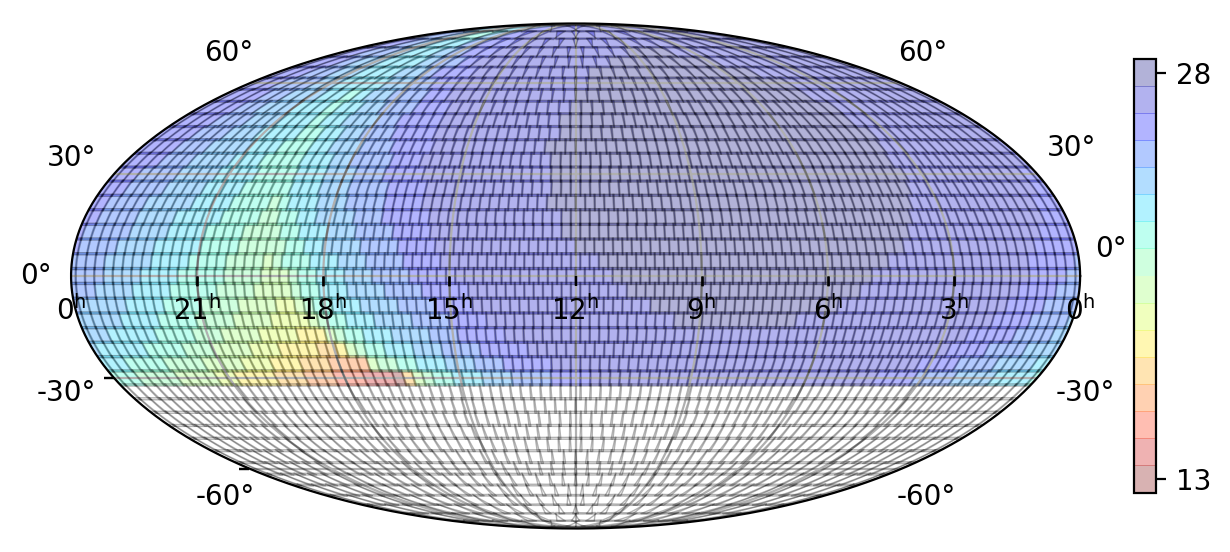
\includegraphics[height=190pt]{images/survey_sims/365_1N4_lite.png}
    \end{center}
    \caption[All-sky survey simulation results: 1N4 system]{
        All-sky survey simulation coverage map for a 1N4 system, as currently deployed on La Palma. Tiles are coloured by the number of times they were observed over the 365 simulated nights. Tiles in white are those not visible from the northern site.
    }\label{fig:survey_sim_1n4}
\end{figure}

\begin{figure}[p]
    \begin{center}
        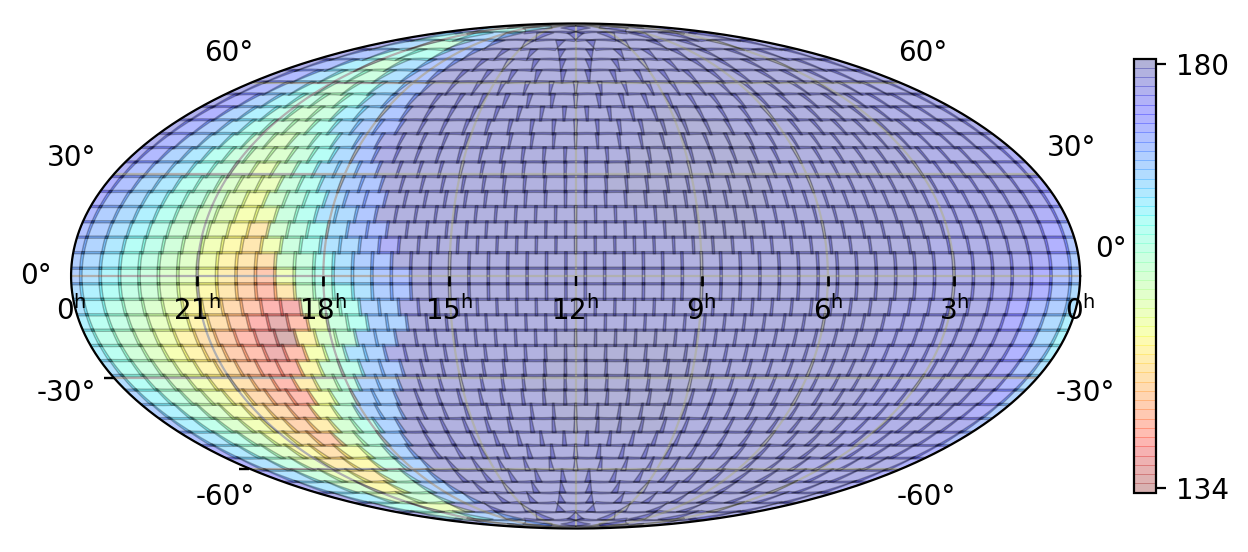
\includegraphics[height=190pt]{images/survey_sims/365_2N8+2S8_lite.png}
    \end{center}
    \caption[All-sky survey simulation results: 2N8+2S8 system]{
        All-sky survey simulation coverage map for a 2N8+2S8 system, the ultimate design goal of the GOTO collaboration. Note the colour scale has changed from \aref{fig:survey_sim_1n4}, the grid has changed to the GOTO-8 tiles and the region which was previously not visible from just the north has been filled in.
    }\label{fig:survey_sim_2n8+2s8}
\end{figure}

\begin{table}[t]
    \begin{center}
        \begin{tabular}{c|cc|c|c|c} % chktex 44
            \multirow{2}{*}{System} &
            \multicolumn{2}{c|}{Fraction of sky observed} &
            No.\ of times &
            Mean cadence &
            {\small Mean airmass}
            \\
            &
            each night &
            over 1y &
            tiles observed &
            (days) &
            observed
            \\
            \midrule
            1N4* & 4.3\%--6.5\% & 76.5\% & 26 (13--28) & $10.0\pm1.8$ & $1.6\pm0.4$ \\
            &&&&&\\
            1N4 & 4.3\%--6.4\% & 76.5\% & 26 (13--28) & $10.1\pm1.8$ & $1.6\pm0.3$ \\
            1N8 & 9.5\%--14.0\% & 74.2\% & 58 (34--62) & $4.6\pm0.7$ & $1.6\pm0.4$ \\
            2N8 & 19.0\%--28.1\% & 74.2\% & 117 (68--123) & $2.3\pm0.4$ & $1.6\pm0.4$ \\
            &&&&&\\
            1N8+1S8 & 23.2\%--24.1\% & 99.9\% & 87 (67--91) & $3.4\pm0.3$ & $1.5\pm0.4$ \\
            2N8+1S8 & 33.0\%--37.3\% & 99.9\% & 130 (98--138) & $2.3\pm0.2$ & $1.6\pm0.4$ \\
            2N8+2S8 & 46.3\%--48.1\% & 99.9\% & 173 (134--180) & $1.7\pm0.1$ & $1.5\pm0.4$ \\
            &&&&&\\
            2N8+2K8 & 46.8\%--48.3\% & 99.8\% & 174 (134--181) & $1.7\pm0.1$ & $1.6\pm0.4$ \\
        \end{tabular}
    \end{center}
    \caption[All-sky survey simulation results summary table]{
        Summary of all-sky survey simulation results. The first 1N4 simulation, marked with an asterisk (*), was the only one carried out using the full scheduler and database system; all the other simulations used the `lite' script. The fraction of the sky observed each night is given as a range over the course of a year, as well as the total fraction of the sky observed over the whole year. The number of times each tile was observed is given as an average over all tiles observed and, in parenthesis, the minimum and maximum. The mean cadence between observations of each tile is also given, along with the mean airmass of each observation, over the whole year.
    }\label{tab:survey_sim_results}
\end{table}

\end{colsection}

% ~~~~~~~~~~~~~~~~~~~~

\subsection{Analysis of simulation results}
\label{sec:survey_sim_analysis}
\begin{colsection}

The results of the all-sky survey simulations show, as expected, that the greatest benefit to the survey cadence comes from increasing the number of telescopes at each site. \aref{fig:survey_sim_results} plots the change in mean cadence and fraction of the sky observed each night for the planned stages of GOTO deployment.

\begin{figure}[t]
    \begin{center}
        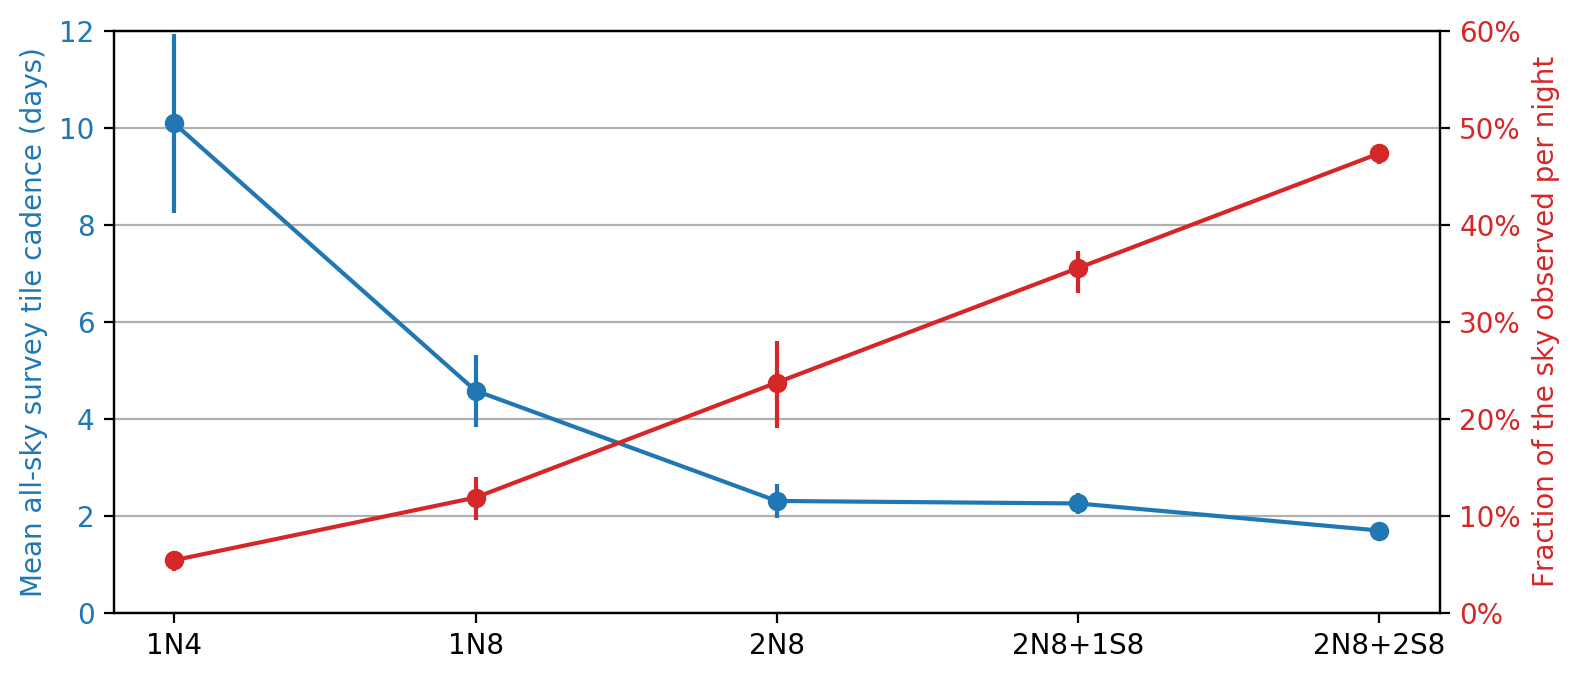
\includegraphics[width=\linewidth]{images/survey_sims/results.png}
    \end{center}
    \caption[Tile cadence and nightly sky observation for different GOTO systems]{
        Mean tile cadence (\textcolorbf{NavyBlue}{blue}) and fraction of the sky observed each night (\textcolorbf{Red}{red}) for five deployment stages of the GOTO system. Error bars on the cadence show the standard deviation for all of the tiles observed across the sky, while the error bars on the observed fraction show the minimum and maximum nightly observed fraction arising from differing night lengths throughout the year.
    }\label{fig:survey_sim_results}
\end{figure}

The improvement in tile observation cadence roughly follows the expected trend that doubling the instantaneous field of view would double the number of observations carried out in one night, and therefore halve the time between observations of a given tile. With the current GOTO-4 system (1N4) the simulations predict approximately 10 days between tile observations, reducing to approximately 5 days with the upgrade to the full GOTO-8 system (1N8) and then halving again to 2.5 days with the addition of the second GOTO-8 telescope on La Palma (2N8). Adding a single GOTO-8 telescope in Australia (2N8+1S8) will leave the tile cadence effectively unchanged, which is simply a matter of geometry. Adding a site in Australia increases the total amount of the sky that is visible over the year from roughly 75\% to almost 100\%, an increase of one third, and adding one more GOTO-8 telescope in the south corresponds to a one third increase in observing capability. Therefore the overall efficiency remains the same as in the 2N8 case. Adding the second telescope in Australia correspondingly decreases the cadence further; as this increases the overall instantaneous field of view by one third the cadence is reduced by a third, from 2.5 to 1.66 days.

As also shown in \aref{fig:survey_sim_results}, the increase in the fraction of the sky observed each night as more telescopes are added is fairly linear. The variation over the course of the year, shown by the error bars, comes from seasonal variation in the length of then night; the variation increases as more telescopes are added in the north but is then reduced to effectively zero with equal numbers of telescopes in both hemispheres.

Together, the sky-survey simulations confirm that having more telescopes decreases the survey cadence, as would be expected. Having a fast all-sky survey is critical for rapidly detecting candidate sources to gravitational-wave events, so it is necessary to consider the results of both sets of simulations together. Counter to the conclusions from \aref{sec:gw_sims}, the simulations in this section suggest it would not necessarily be best to prioritise adding a telescope in the south compared to adding a second telescope in the north. While going from the 1N8 case to the 2N8 case makes very little difference to the number of gravitational-wave events that can be observed, it would half the survey cadence from 4.6 days to 2.3, thereby making it far easier to identify candidates for the events that are visible. The decision of what order to deploy the GOTO telescopes therefore will come down to more practical considerations. Having any telescopes in the southern hemisphere will increase the number of possible gravitational-wave sources that could be observed, but without a high-cadence sky survey identifying the counterpart will be much more difficult.

Overall, the two sets of simulations together suggest that the proposed full GOTO network, the ``2N8+2S8'' system, should expect to observe the position of over of 75\% of gravitational-wave sources within 24 hours, and over 50\% within 12 hours. On average there should be a reference image taken of the same position within the past 1.7 days, which will greatly help narrowing in down potential candidate sources. When fully deployed GOTO would therefore be a powerful system for rapidly finding counterparts to gravitational-wave detections.

\newpage

\end{colsection}

% ~~~~~~~~~~~~~~~~~~~~

\subsection{Comparison of simulations to real observations}
\label{sec:survey_sim_150}
\begin{colsection}

The results of the 1N4 simulation can be compared to the real observations carried out by the existing telescope on La Palma, in order to confirm how good a model it is of the real system. The current phase of the GOTO project began on the night of the 21st of February 2019 (see \aref{sec:timeline}); this was the first night of fully robotic observations with the set of four unit telescopes, and marks the start of the ongoing all-sky survey. The first 5 months of observations span 150 days up to the night ending on the 21st of July, and this provides the benchmark to compare with simulations of the same period.

\begin{figure}[p]
    \begin{center}
        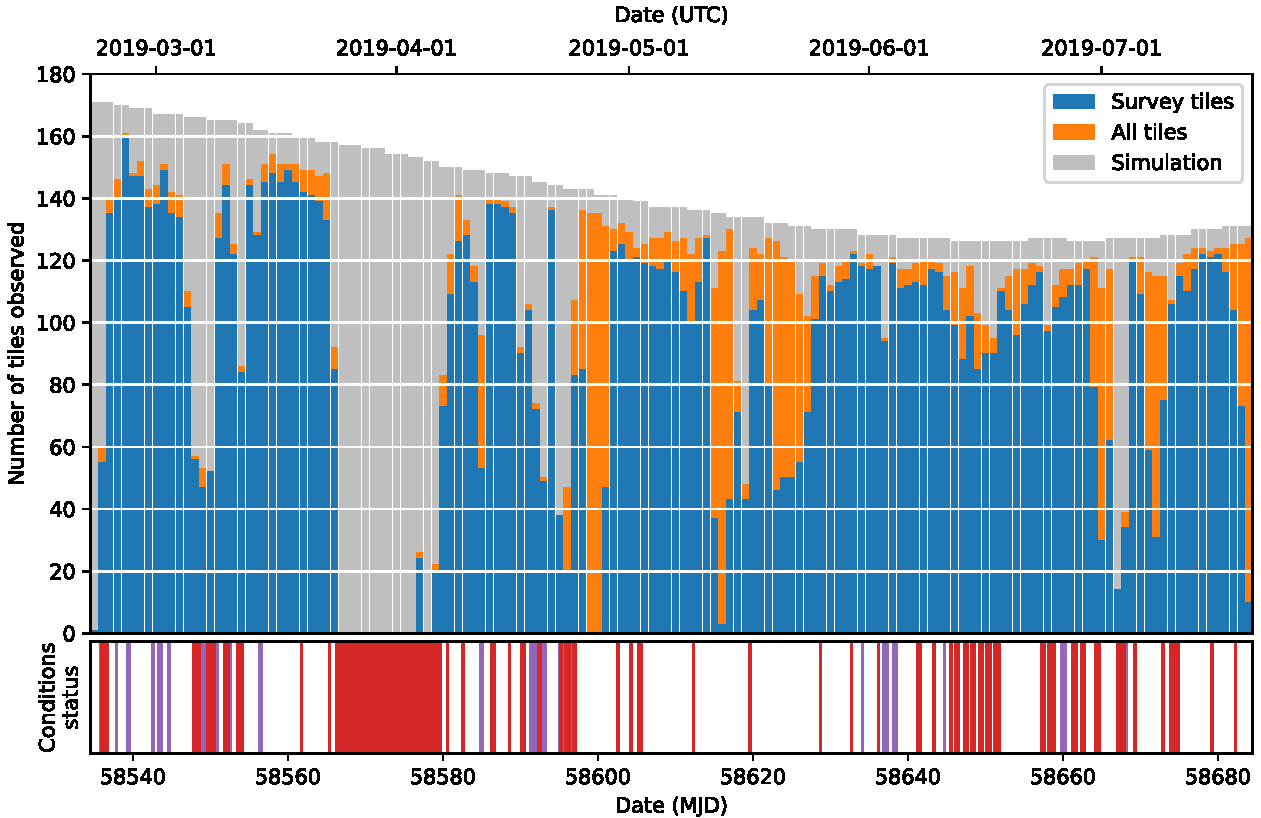
\includegraphics[width=\linewidth]{images/150.pdf}
    \end{center}
    \caption[Observations carried out in the first 150 days of the all-sky survey]{
        Observations carried out in the first 150 days of the current all-sky survey. The number of observations each night is shown in the upper plot, with the number of all-sky survey tiles observed shown in \textcolorbf{NavyBlue}{blue}, and any extra observations (of gravitational-wave events, GRB triggers or manually-inserted pointings) shown in \textcolorbf{Orange}{orange}. The background \textcolorbf{Gray}{grey} bars show the number of tiles observed on the same nights by the 1N4 survey simulation. The lower ``barcode'' plot shows the periods when the conditions flags were recorded as bad, either due to weather (\textcolorbf{Red}{red}) or hardware errors (\textcolorbf{Purple}{purple}).
    }\label{fig:150}
\end{figure}

\aref{fig:150} shows the number of tiles observed each night by the real GOTO on La Palma and the corresponding 1N4 simulation, restricted to the first 150 days. Over the 5-month period, 16146 on-grid observations were carried out by the telescope on La Palma, of which 85\% were survey pointings, and over the same period the simulation produced 21300 observations. The simulated observations can be considered the idealised case, and the real observations carried out differ from simulation in three ways.

First, the real system on La Palma is affected by bad conditions which prevent observations from being taken, shown in \aref{fig:150} by the red and purple bars below the main plot. There was one particularly bad period in late March and early April when the dome could not open for over a week. The simulations do not currently include the effects of bad weather, although the code exists to simulate periods of bad conditions and future simulations could include the real weather conditions over the same period. There were also other reasons for observations to be stopped on some nights, for example switching to manual mode to carry out calibration tests or on-site work.

Secondly, the real system had to deal with multiple distractions from observing the all-sky survey. The orange bars in \aref{fig:150} show non-survey observations, which take up a significant amount of time (15\% of all observations). Some nights are almost entirely orange, corresponding to LVC gravitational-wave triggers with particularly large skymaps visible from La Palma (see \aref{sec:gw_results}). These include S190425z and S190426c in late April, multiple events during May and S190720a just before the end of the period in mid-July. Other orange patches represent observations of smaller gravitational-wave skymaps, gamma-ray burst triggers, or other manually-inserted targets; these were also not considered in the sky-survey simulations.

Finally, there is still a regular offset in \aref{fig:150} between the number of real observations taken in nights with clear conditions and the number predicted by the simulations. This discrepancy is due to the values used within the simulation for camera readout and slew time not matching up precisely with the actual times; future simulations will need to be calibrated more accurately against real data.

\aref{fig:survey_real_150} shows the sky coverage map for the real observations in the first 150 days, while \aref{fig:survey_sim_1n4_150} shows the same for the 1N4 simulation. The real sky coverage is very similar in extent to the simulations: the real observations cover 2135 of the 2913 GOTO-4 grid tiles at least once while the simulation covers 2187. The reason for the small discrepancy is that initially the real system used an altitude limit of \SI{35}{\degree} for the all-sky survey, which was lowered to \SI{30}{\degree} in May. This change is visible in the bottom row of tiles in \aref{fig:survey_real_150}. The simulations all assume a constant \SI{30}{\degree} limit.

The major difference in the coverage between the real and simulated results is in the number of times each tile as observed. \aref{fig:survey_real_150} shows the most a real tile was observed was nine times, while \aref{fig:survey_sim_1n4_150} shows that the simulated results included up to 13 observations of a single tile. The mean tile cadence of the real observations is $14\pm4$, compared to $10\pm2$ from the 1N4 simulation. It is clear that future simulations need to take into account the time lost to weather and other non-survey observations in order to accurately predict the output of the real system. Overall though, aside from the constant offset visible in \aref{fig:150}, the simulations do seem to provide a reasonable approximation of what GOTO could observe in this idealised case.

\begin{figure}[p]
    \begin{center}
        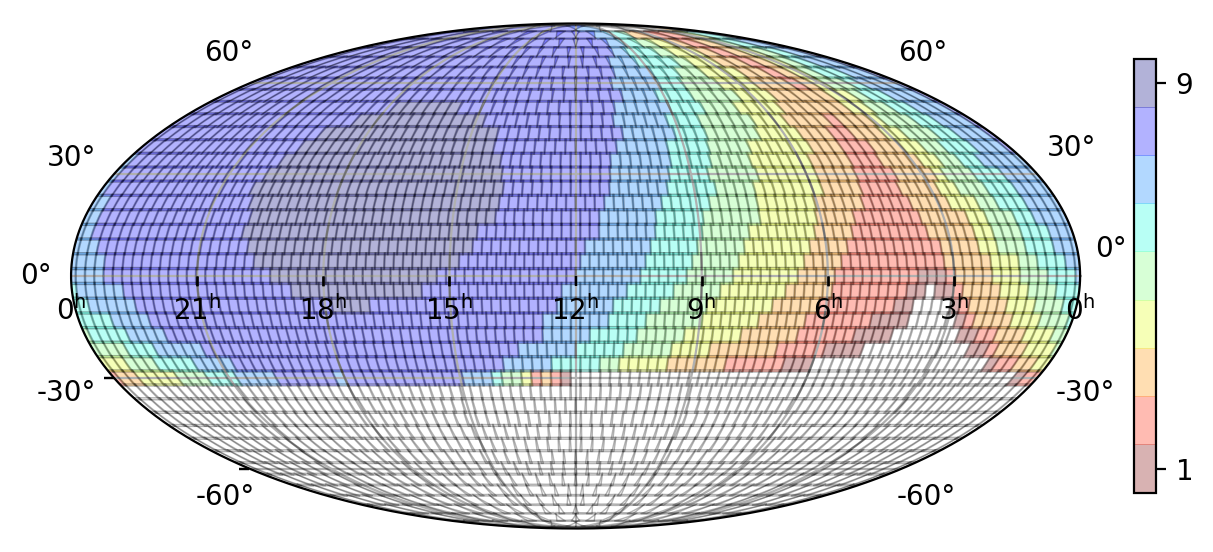
\includegraphics[height=190pt]{images/survey_sims/150_1N4_real.png}
    \end{center}
    \caption[Real survey observations over 150 days]{
        Real all-sky survey map of observations over the first 150 days, from 21st February to 21st July 2019. Tiles are coloured by the number of times they were observed during this period, and tiles in white were not observed.
    }\label{fig:survey_real_150}
\end{figure}

\begin{figure}[p]
    \begin{center}
        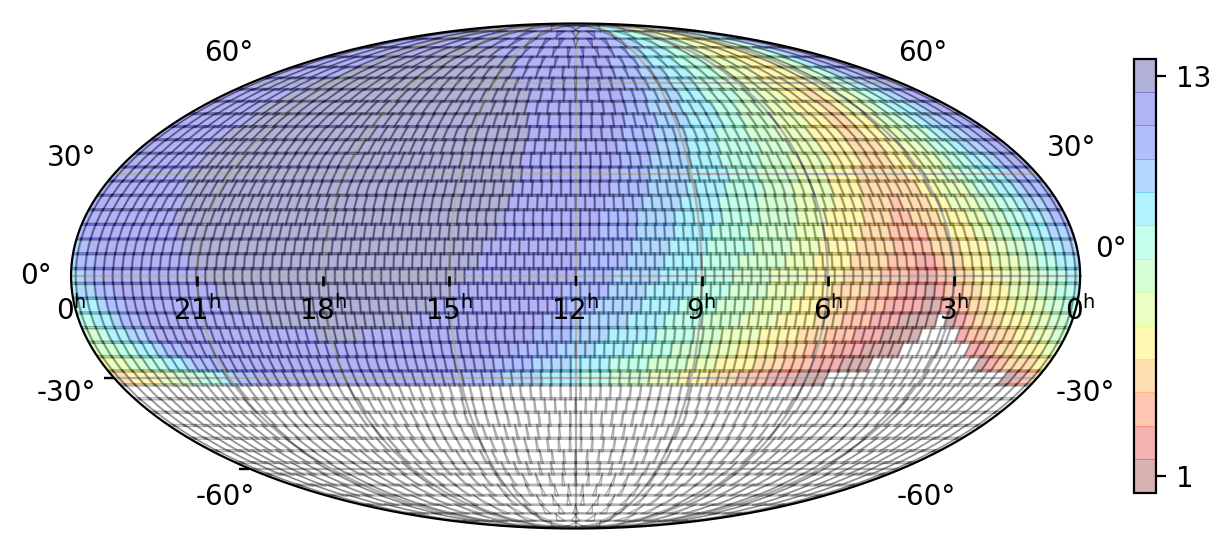
\includegraphics[height=190pt]{images/survey_sims/150_1N4_lite.png}
    \end{center}
    \caption[1N4 survey simulation observations over 150 days]{
        Simulated 1N4 all-sky survey map of observations over the first 150 days. Compare to \aref{fig:survey_sim_1n4} for the coverage over the entire 1-year simulation.
    }\label{fig:survey_sim_1n4_150}
\end{figure}

\clearpage
\newpage

\end{colsection}

% ~~~~~~~~~~~~~~~~~~~~

\subsection{An alternative, meridian-limited sky survey method}
\label{sec:survey_sim_meridian}
\begin{colsection}

One of the problems with the current scheduling system for the all-sky survey is that it leads to observations being carried out at low airmasses. Due to how the scheduler ranks tiles (see \aref{sec:ranking}), when all of the visible survey tiles have been observed the same number of times the scheduler will then chose between them based on the airmass tiebreak parameter (unlike tiles linked to skymaps all survey tiles have equal weights, so the tiebreaking algorithm developed in \aref{sec:scheduler_tiebreaker} is simplified). This results in the scheduler always selecting tiles as soon as they rise if they have been observed fewer times than any others currently visible, and this means survey tiles are often observed at low airmasses leading to poor data quality.

One possible method to fix this problem and improve the data quality is to implement stricter limits when observing survey tiles. This should not be based on altitude or airmass, because that would exclude tiles close to the site declination limits (such as near the north celestial pole from La Palma) which could never rise above the limit. Instead, observations should be limited based on distance from the observer's meridian, which in practice limits the target's hour angle. Limiting observations by hour angle defines a strip surrounding the observer's meridian within which survey tiles are valid and outside of which they are not.

In order to see the consequences of this method several simulations were carried out using the 1N4 system, but modified to limit the hour angle of each target. The results of the simulations are given in \aref{tab:survey_sim_meridian}, for different hour angle limits and the unlimited case for comparison. \aref{fig:survey_sim_airmass_365} shows the change in distribution of airmasses between the existing unlimited method and when restricting observations to a \SI{20}{\degree} wide strip ($\pm\SI{10}{\degree}$) around the observer's meridian. \aref{fig:survey_sim_airmass_normal} shows the mean airmass each tile is observed in the first month of a survey using the existing method, while \aref{fig:survey_sim_airmass_meridian} shows the same thing but for a simulation using the hour angle limit.

By restricting observations to be closer to the observer's meridian the mean airmass of the observations is decreased, as expected. This is shown by the mean airmasses in \aref{tab:survey_sim_meridian} but is even clearer in the distributions shown in \aref{fig:survey_sim_airmass_365}. The optimal value of the hour angle limit will depend on several factors, including the number of telescopes being used (as the instantaneous field of view increases, the tiles within the meridian strip will be observed faster, and so the hour angle limit should be increased).

A side effect of this method is that, as the width of the meridian strip is decreased and the effective visible sky is reduced, each tile within the strip is observed more often, and therefore the mean cadence decreases. However, this also restricts the overage area and leads to fewer unique tiles being observed, as shown in \aref{fig:survey_sim_airmass_meridian}. From \aref{tab:survey_sim_meridian} the fraction of sky observed within a single month reduces from almost 60\% using the unlimited method to almost to 40\% with the strictest hour angle limit. This would have a knock-on effect on the effectiveness of the sky survey, as although lower-airmass observations are desirable, so are more recent observations of the tiles for difference imaging. In practice it might be necessary to have two concurrent surveys, one optimised for minimum airmass and the other optimised for cadence.

\begin{table}[t]
    \begin{center}
        \begin{tabular}{c|cc|c|c|c} % chktex 44
            Survey &
            \multicolumn{2}{c|}{Fraction of sky observed} &
            Mean cadence &
            Mean observed
            \\
            method &
            1st month &
            whole year &
            (days) &
            airmass
            \\
            \midrule
            Meridian  \SI{\pm5}{\degree} & 39.4\% & 76.5\% &  $6.2\pm0.5$ & $1.2\pm0.2$ \\
            Meridian \SI{\pm10}{\degree} & 41.3\% & 76.5\% &  $6.6\pm0.7$ & $1.2\pm0.3$ \\
            Meridian \SI{\pm30}{\degree} & 48.5\% & 76.5\% &  $7.9\pm0.8$ & $1.3\pm0.3$ \\
            Meridian \SI{\pm45}{\degree} & 53.3\% & 76.5\% &  $8.8\pm0.9$ & $1.3\pm0.3$ \\
            No limit                     & 57.0\% & 76.5\% & $10.1\pm1.8$ & $1.6\pm0.3$ \\
        \end{tabular}
    \end{center}
    \caption[Comparison of survey simulations using a meridian limit]{
        Comparison of 1N4 survey simulations using different meridian limits.
    }\label{tab:survey_sim_meridian}
\end{table}

\begin{figure}[p]
    \begin{center}
        \begin{minipage}[t]{0.49\linewidth}\vspace{10pt}
            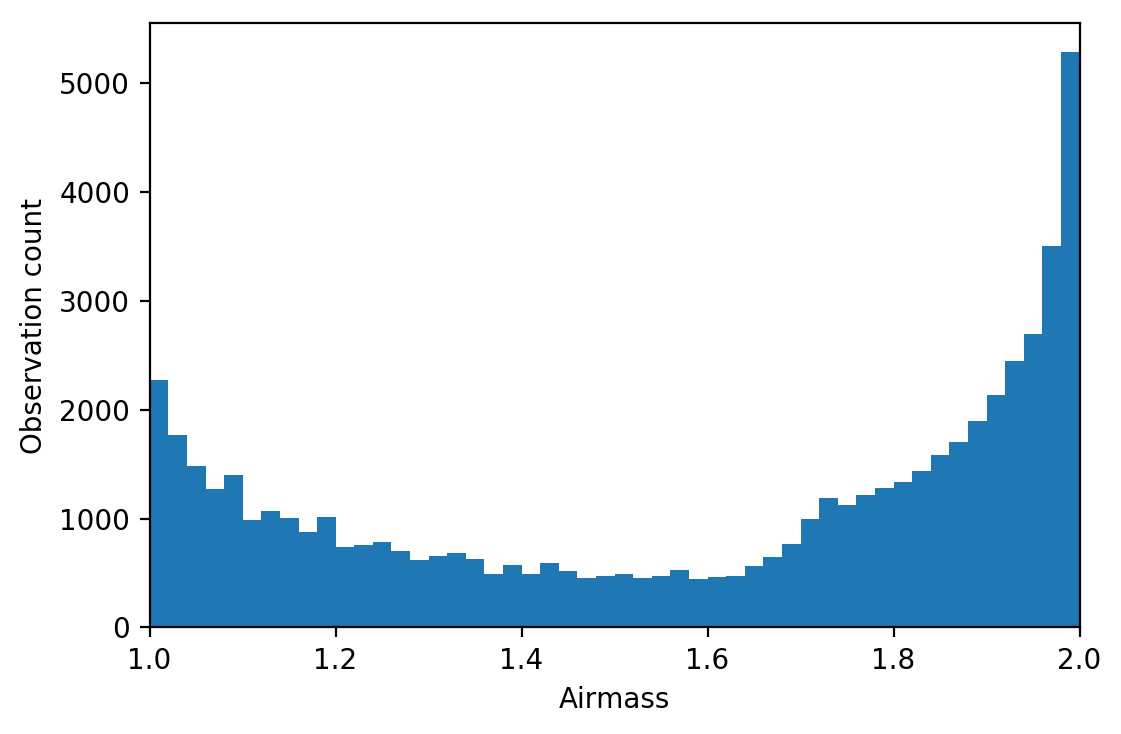
\includegraphics[height=140pt]{images/survey_sims/365_1N4_lite_airmass3.png}
        \end{minipage}
        \begin{minipage}[t]{0.49\linewidth}\vspace{10pt}
            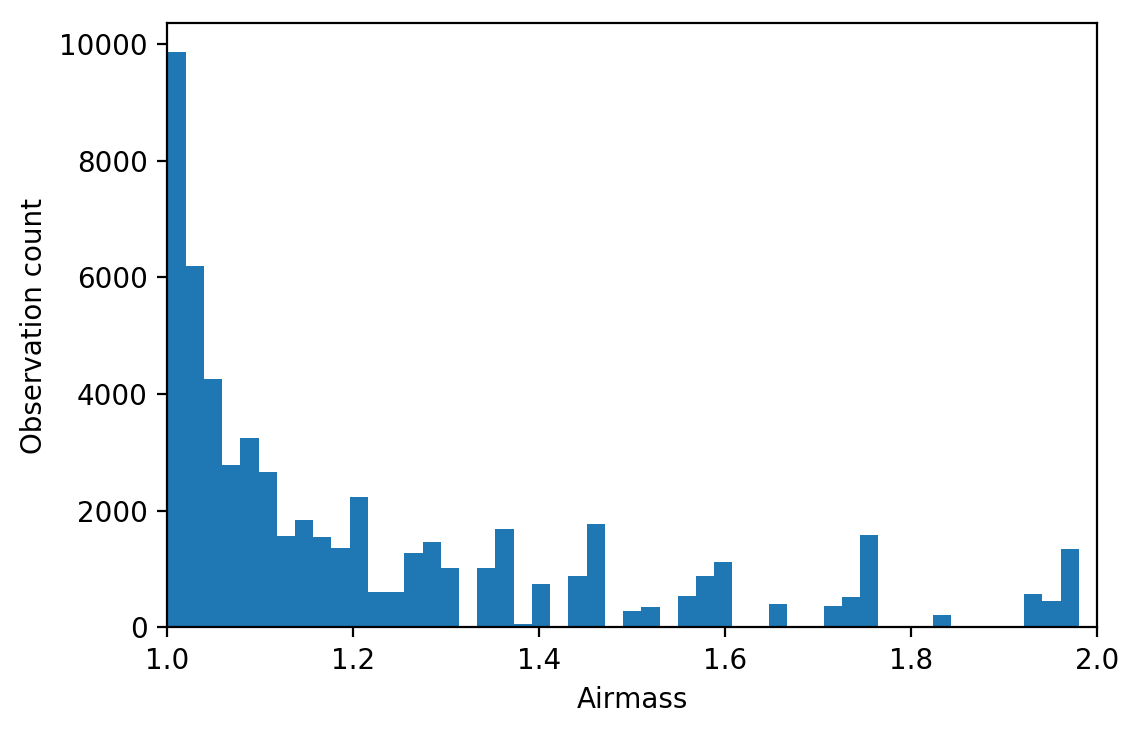
\includegraphics[height=140pt]{images/survey_sims/365_1N4_meridian_airmass3.png}
        \end{minipage}
    \end{center}
    \caption[Airmass distribution over a year of observations]{
        Airmass distribution over a year of observations with the 1N4 system, for the normal unlimited case (left) and limited to the observer's meridian $\pm\SI{10}{\degree}$ (right).
    }\label{fig:survey_sim_airmass_365}
\end{figure}

\begin{figure}[p]
    \begin{center}
        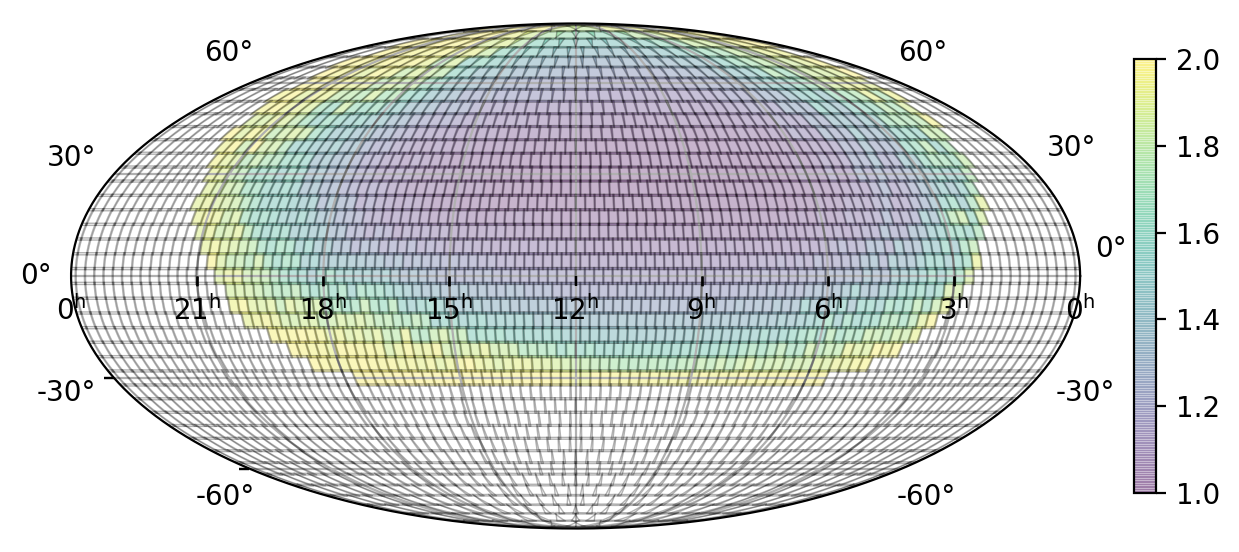
\includegraphics[width=0.7\linewidth]{images/survey_sims/30_1N4_lite_airmass.png}
    \end{center}
    \caption[Mean observation airmasses for the 1N4 survey simulation]{
        Mean observation airmasses for the first month of the 1N4 survey simulation, with no hour angle limit.
    }\label{fig:survey_sim_airmass_normal}
\end{figure}

\begin{figure}[p]
    \begin{center}
        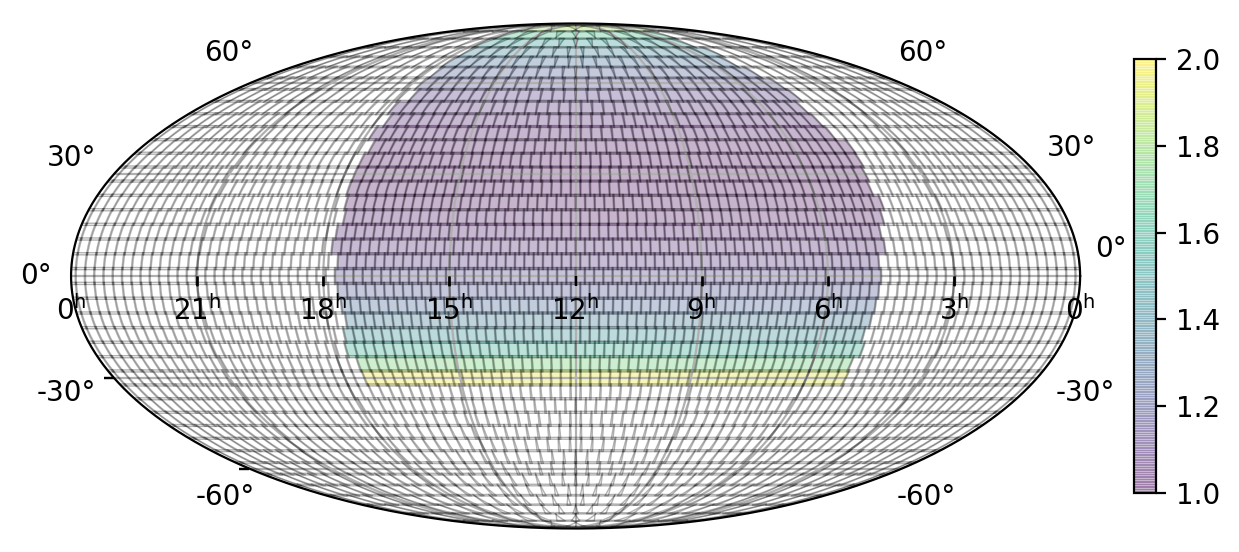
\includegraphics[width=0.7\linewidth]{images/survey_sims/30_1N4_meridian_airmass.png}
    \end{center}
    \caption[Mean observation airmasses using the meridian scanning method]{
        Mean observation airmasses for the first month of a survey using the meridian scanning method, restricting observations to tiles within $\pm\SI{10}{\degree}$ of the observer's meridian. Using the hour angle limit it possible to optimise the airmass of observations, but at the cost of sky coverage.
    }\label{fig:survey_sim_airmass_meridian}
\end{figure}

\end{colsection}

% ########################################
